\chapter{Analysis}

\section{Introduction}

Client: Neil Green
Job Description: Owns and manages an Independently run gym
Contact Information: Sweat Gymnasium LLP
					 107a Clay Street
					 Soham
					 Ely
					 Cambridgeshire
					 CB7 5HL

					 Telephone: 01353 721864
					 Email: info@sweatgym.co.uk

\subsection{Client Identification}

My client is an independent gym owner who is struggling to keep track of his members payment details and use of the facilities. He is also my brother in law. He approached me about creating a system for him after I mentioned I needed a client for coursework and he mentioned that he is having issues with clients not paying him since he doesn't have an accurate, reliable system for keeping track of payments. He also has to manage staff members throughout the day and has to manage his business' accounts, which relies a lot on his current system for keeping track of his members payments. His gym has over a 1000 members which he keeps track of using excel spreadsheets. He made these spreadsheets himself so he has a reputable amount of I.T skills (I go more in depth regarding his and his employees I.T abilities in the Constraints section). I have accumulated the information for the following sections via an interview (presented in full in the appendix) and text messages/email and general conversation as I see him and several of his employees quite frequently but don't always have the chance to document the interaction. 

\subsection{Define the current system}

His current system involves using a series of excel spreadsheets to document his clients payment, membership details, personal details and exercise plans. He does this manually by creating new spreadsheets and entering the clients data by hand. His clients give him this data by filling out a membership form and membership agreement and via discussion and another entry form if they need an exercise program made for them. My client uses one spreadsheet (presented in section: Investigation) to keep a record of all the members of the gym including details like their member ID, their contact information and membership details, and another for their payment information (presented in section: Investigation) as well as whether their up to date with these payments. Each member then has their own table which is used to keep track of any exercise routines they may have asked to have planned for them. When the applying member signs up they get given information regarding the gym including payments details so that the can pay via direct debit. Every month the owner checks his mandates to see who has and hasn't made their payment. When a member of the gym leaves all of their information is kept in case they return to their membership in the future. All of the exercise regimes are dated so that it can be referred back to if the member decides they want to change their regime. He then scans these sheets and saves them digitally and uses another physical sheet to document the new regime. A lot of the time he will immediately scan the sheet as members normally request a copy, plus he finds it useful to have a backup especially when dealing with physical forms. All of these spreadsheets and regime forms are kept on the owners workstation computer at the reception desk. Usually he will send the not print the spreadsheets unless he outsources his accounts to another employee or an accountant and he isn't comfortable supplying them with a full digital, or they just find it easier to deal with a physical version. He doesn't keep any of his clients debit/credit card information as all transactions are performed by the members through either direct debit, paying by card at the gym or cash.   

\subsection{Describe the problems}

This system imposes some limitations. First of all, all the processes have to be dealt with manually through spreadsheets without anything other than lack of human error to point out a mistake or notify if someone isn't up to date with payment. This also isn't secure as any piece of information can be changed at any time and to be sure of everything debit mandates would have to be looked over, but even then some clients may have payed by cash and thus wouldn't be recoverable. Their is also the possibility of a computer error that could delete all the documents as they are not backed up anywhere. His gym also now accommodates over 1000 members meaning that he has a large number of spreadsheets for all his clients as well as having his main spreadsheet being exceptionally large meaning the program can lag, especially since the program isn't running on the greatest available hardware. Another issue is that it can be difficult to sort through and search the spreadsheets to find specific information regarding clients, for example if he needs to find they're contact information, excel doesn't have a tool to easily search for that. He also has no easy way to create invoices or just clean organised print outs of any information he needs.

\subsection{Section appendix}

Q. What is your current system?

Our current system involves entering data regarding our clients into excel spreadsheets to keep track of the data we need

Q. And what data is it that you record?

We use the first spreadsheet to record our clients names, contact information, and what membership they have, as well as another for payment details. Each member then has their own table for us to detail any exercise plans that they request for us to create. 

Q. What are the limitations of this?
This system means that everything has to be done manually and I won't know if Iv'e forgotten to enter whether someones paid or not as their is no way for me to know if I forgot to change part of the spreadsheet or if my client is trying not to pay. It also isn't very secure as anyone could edit it easily. The process can also be very time consuming.

Q. Is their any additional data you would like to be recorded in the new system?
I would like to be able to store all of the clients information in one place instead of having to use multiple spreadsheets so I can organise all my data more easily. Though i'm pretty sure I don't need any additional information.

Q. What processes do you normally go through with your current system and how do you implement it?
To use my current system I ask my clients to fill out two forms (presented in the investigation section) and then take the information they filled out and enter them digitally into the appropriate excel spreadsheets.

Q.How would you like to operate the new system?
I would like to be able to operate the system similar to how I operate my current one with me being able to enter information from forms my clients filled out, or perhaps even with digital forms I can email them to fill out.

Q.What Inputs and outputs would your new system need? 
I would like to be able to print out a clients information easily in an organised fashion and also be able to create print outs of any other information I would like, possibly to create an invoice or general report for the client. I would also need some physical forms if possible for my less technically inclined members.

Q. What hardware would this need to run on?
This would be run off a reasonably mid spec laptop purchased four years ago. All I really know is it has an i5 processor.

\begin{figure}[H]
    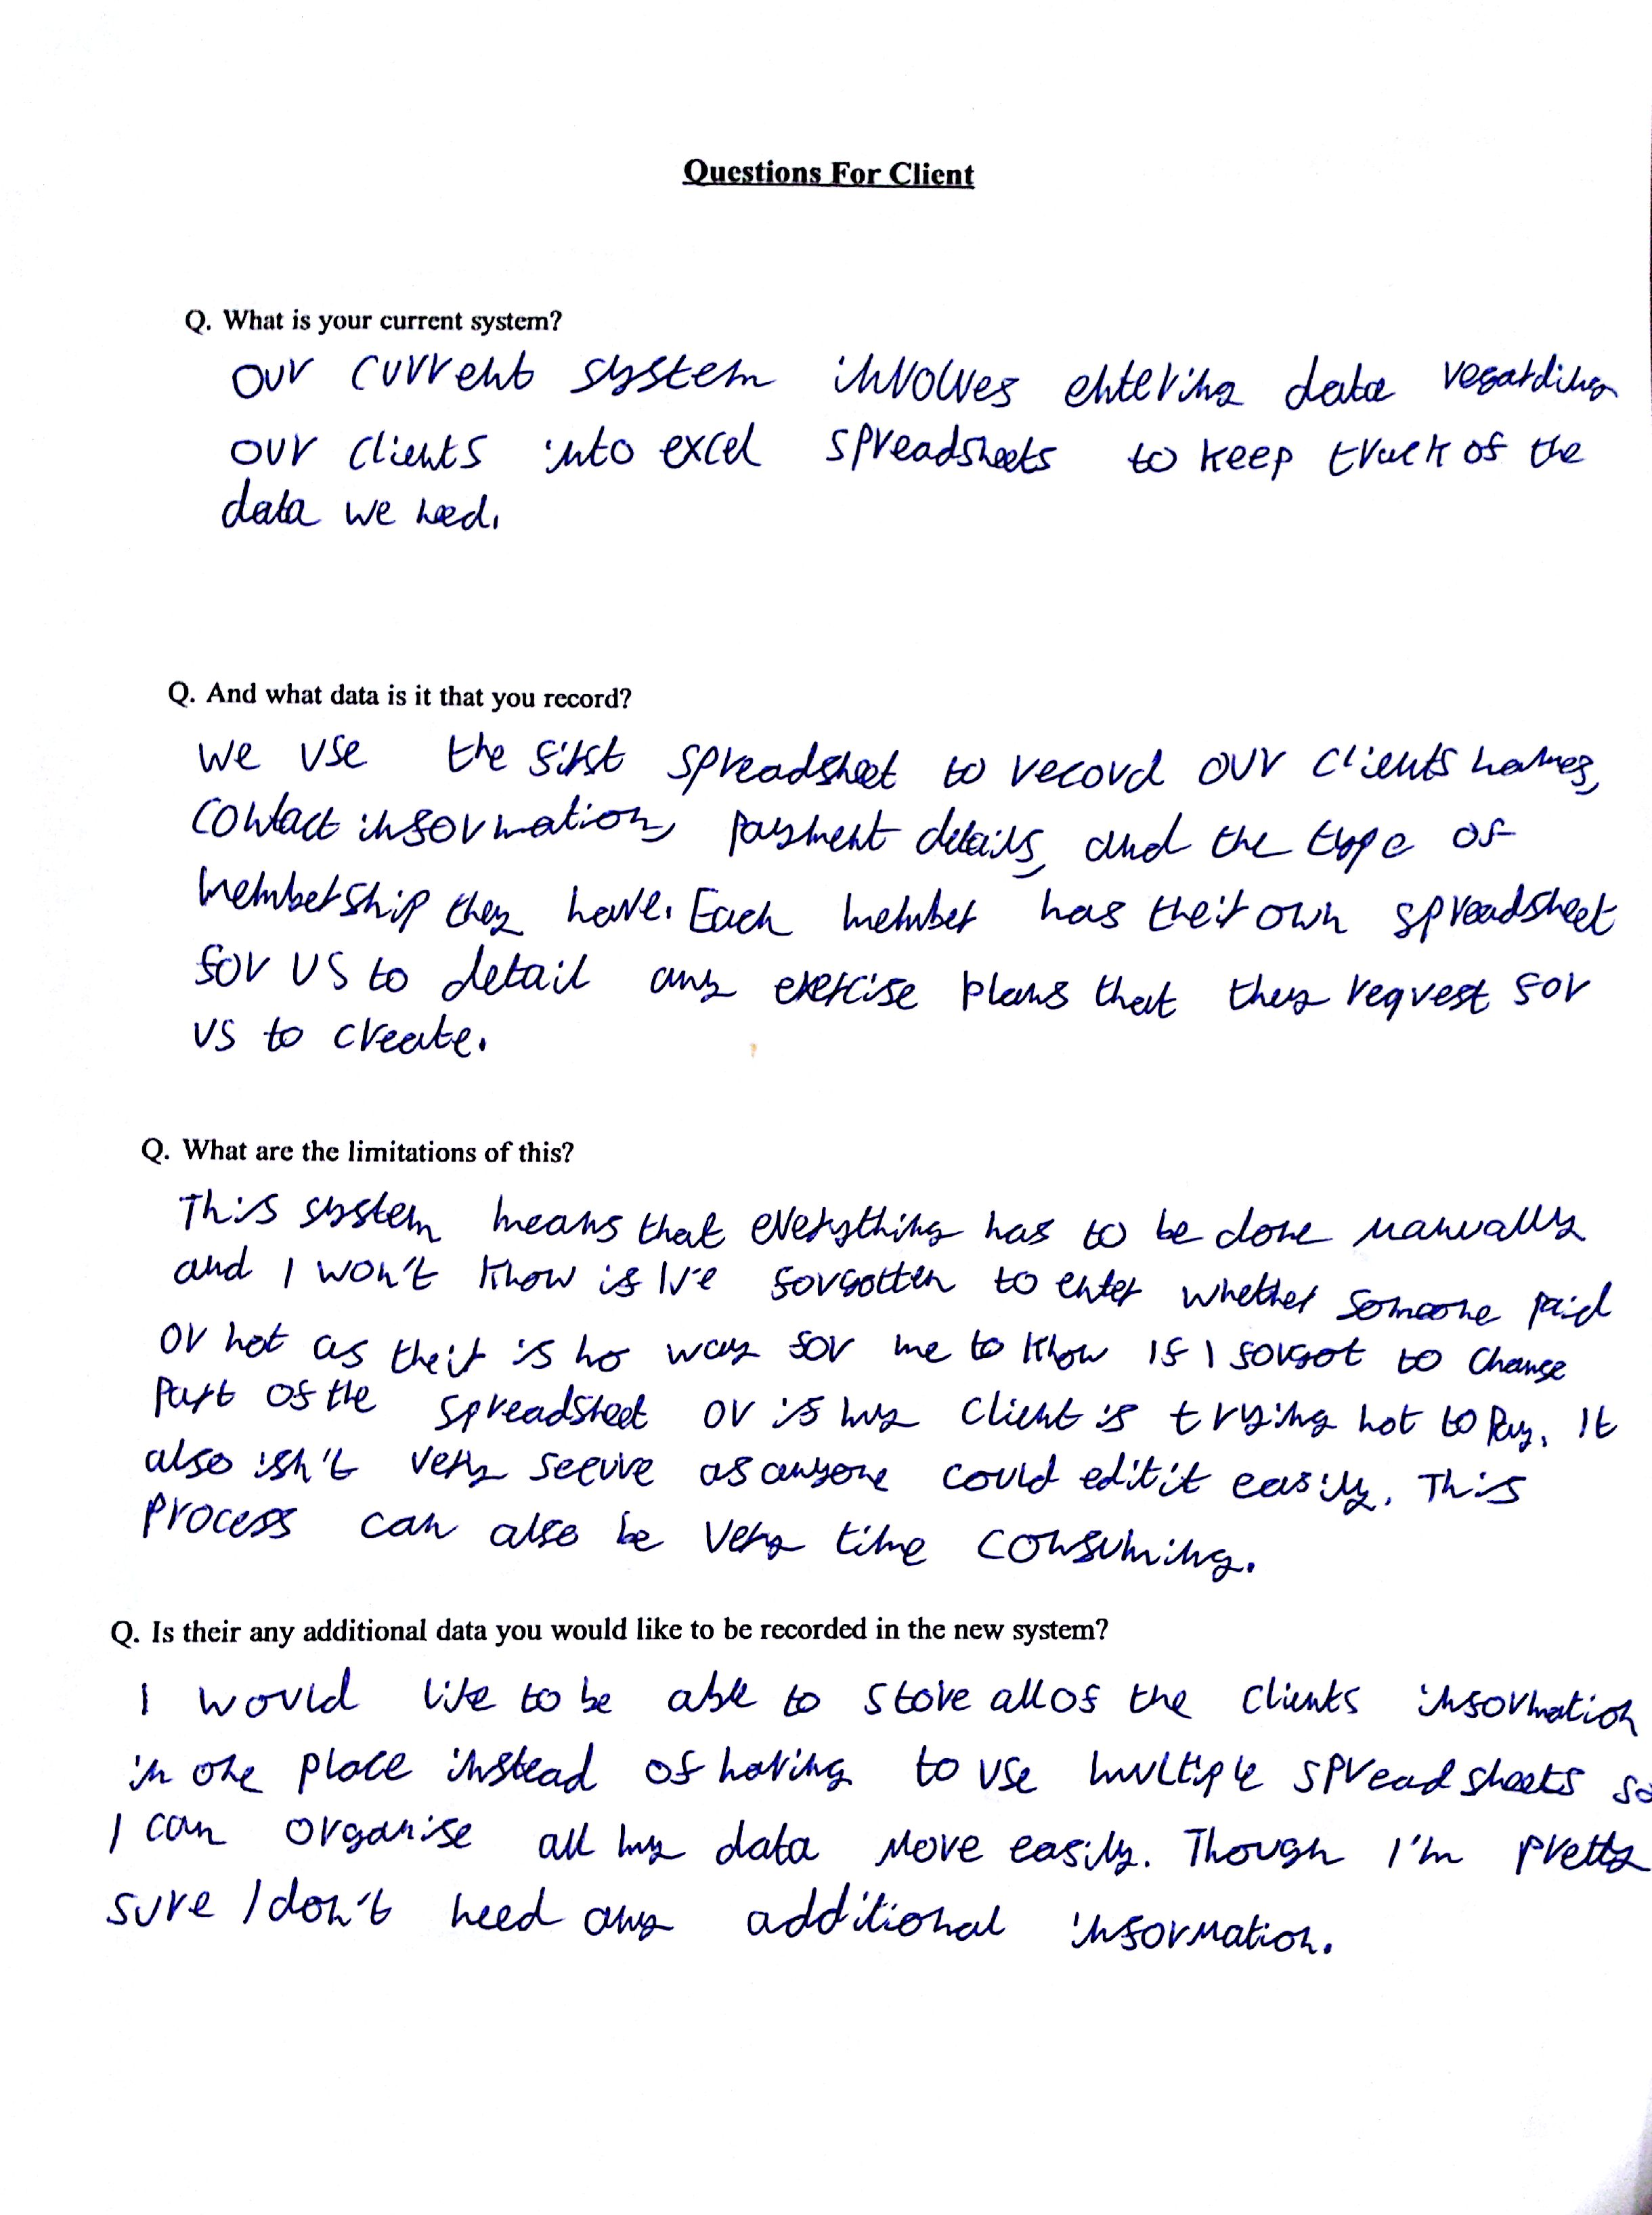
\includegraphics[width=\textwidth]{questionaire 1.jpg}
    \caption{1st page of the questions aksed to my client} \label{fig:1st page of the questions aksed to my client}
\end{figure}
\section{Investigation}

\begin{figure}[H]
    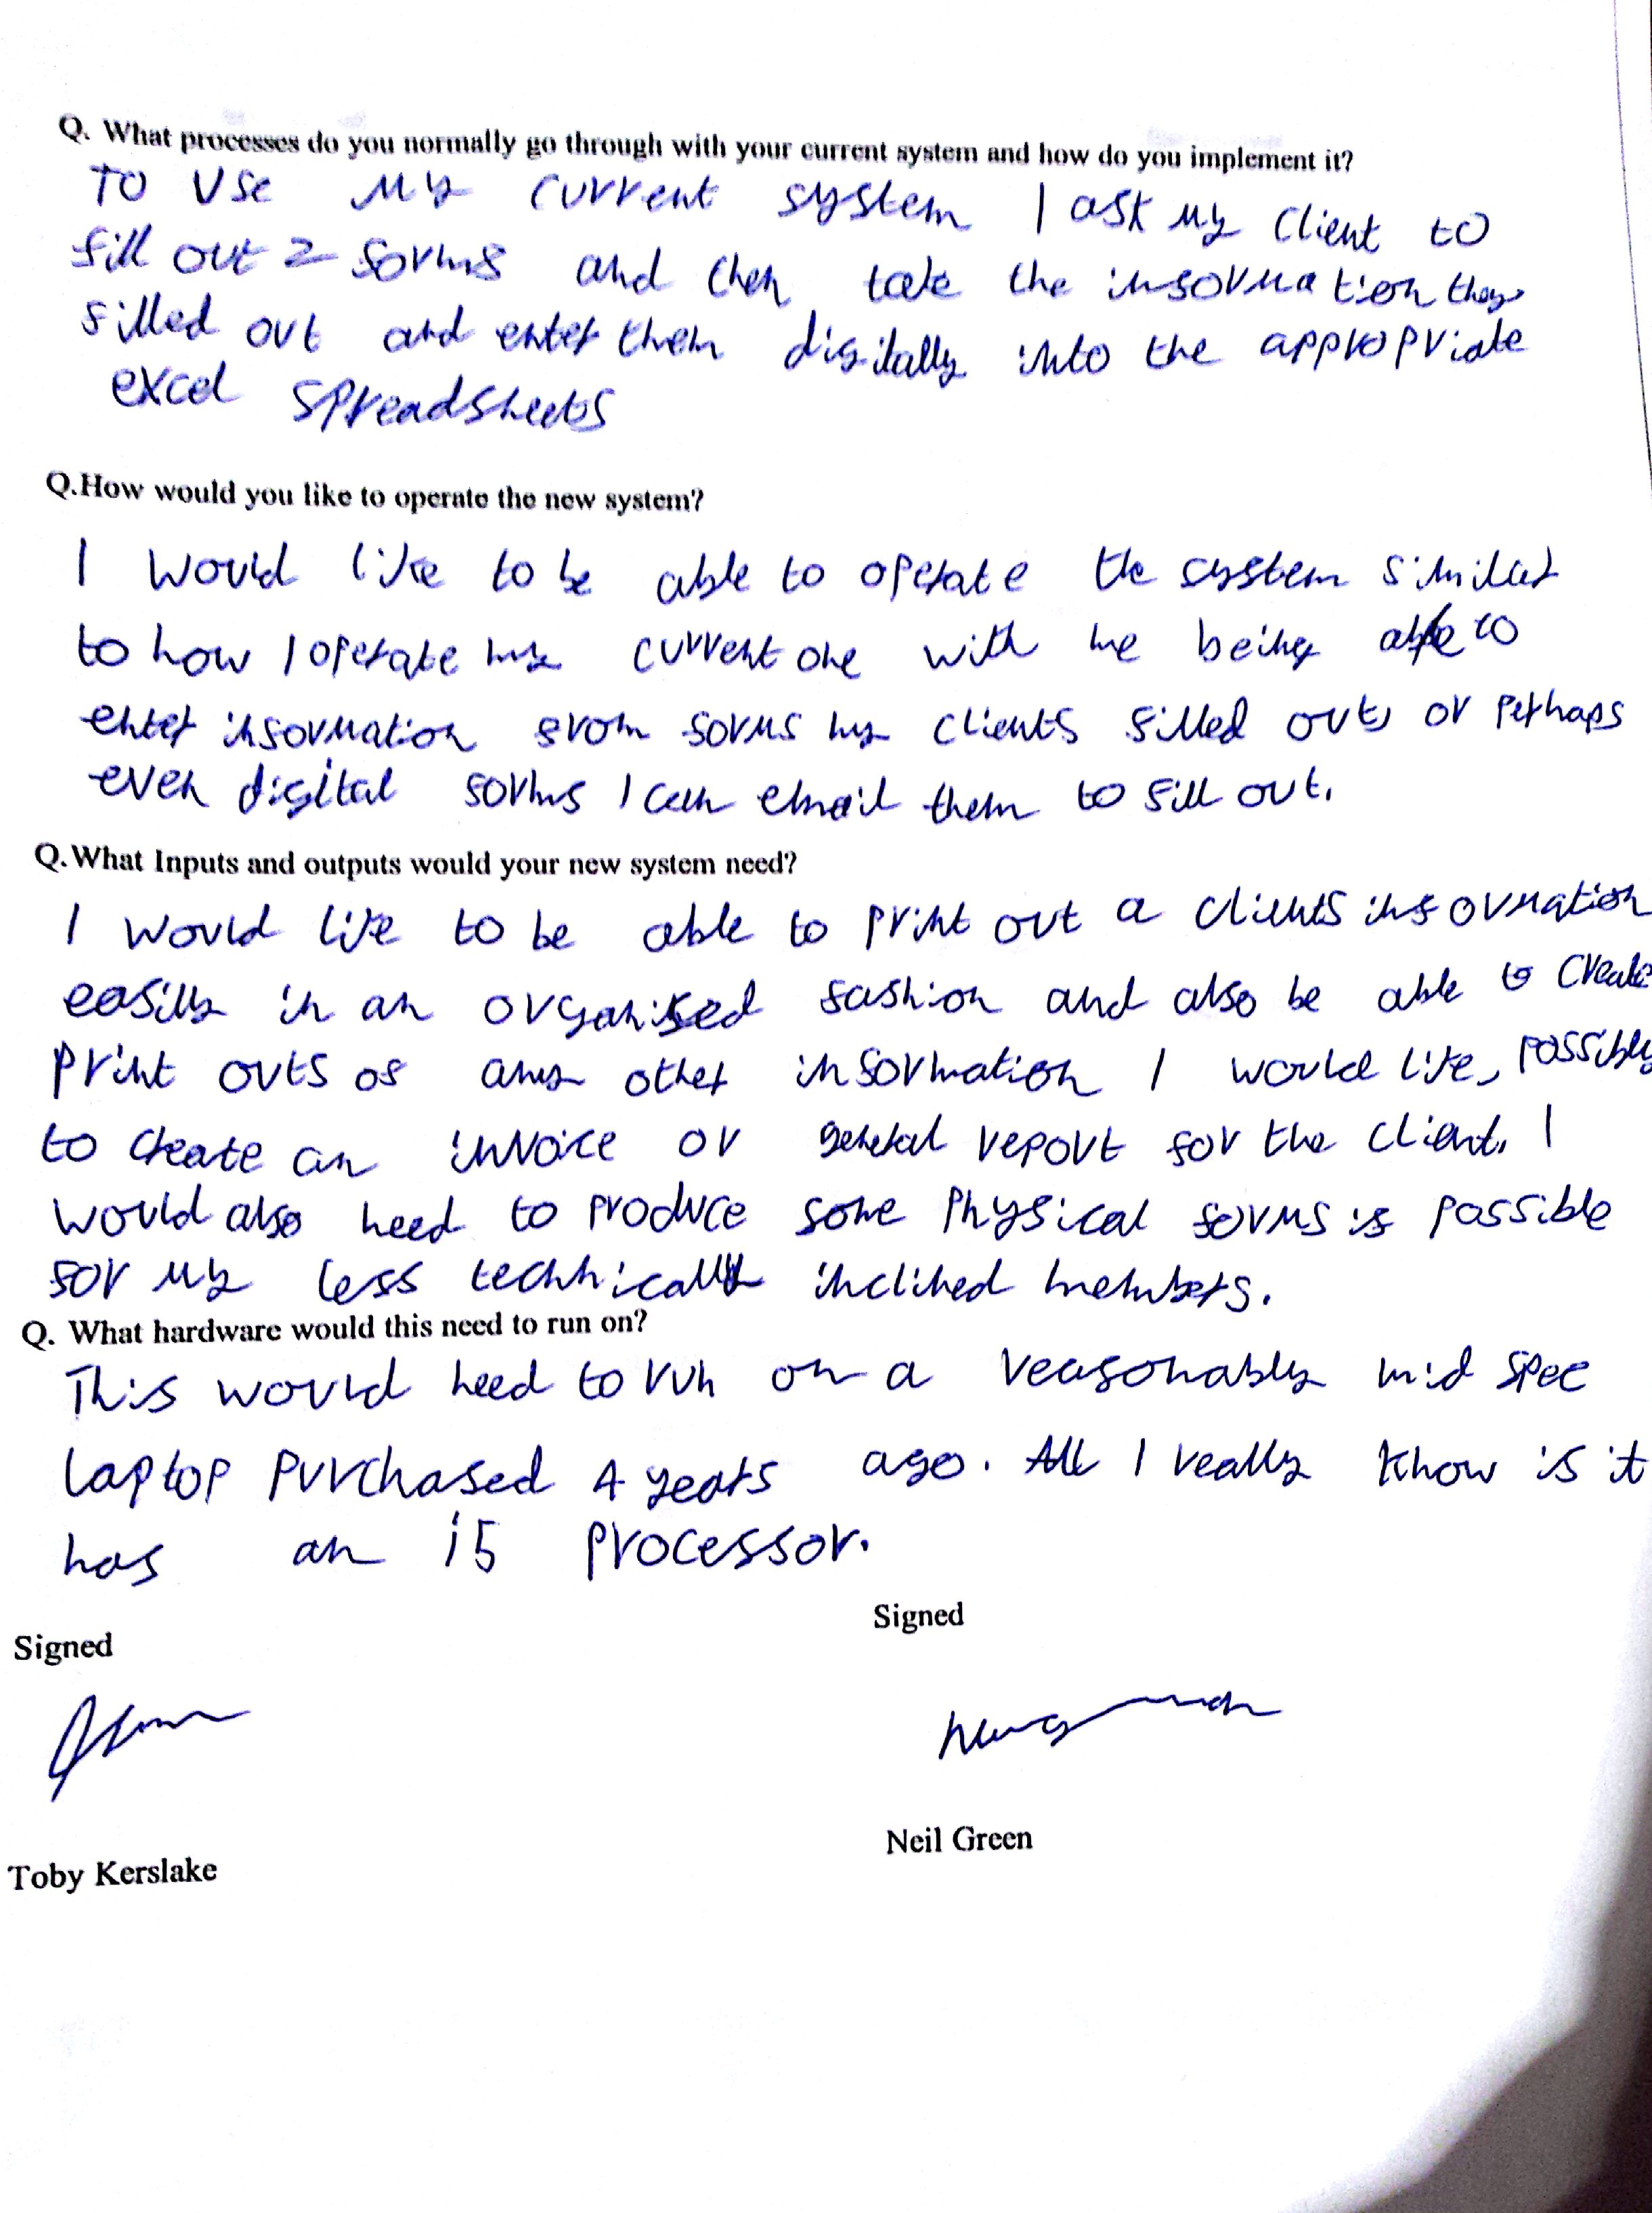
\includegraphics[width=\textwidth]{Questionaire 2.jpg}
    \caption{2nd page of the questions aksed to my client} \label{fig:2nd page of the questions aksed to my client}
\end{figure}
\section{Investigation}

\subsection{The current system}

The current system is made of completely manual functions only using computers for data entry and storing the spreadsheets in which the data is entered. I do my best to explain this system below through the use of hierarchy charts, flowcharts, data flow diagrams and the all the physical and digital forms used in the process.

\subsubsection{Data sources and destinations}

The table below presents all the data curently used in the system, where its come from, where its being stored and gives an example of said data.

\begin{figure}[H]
    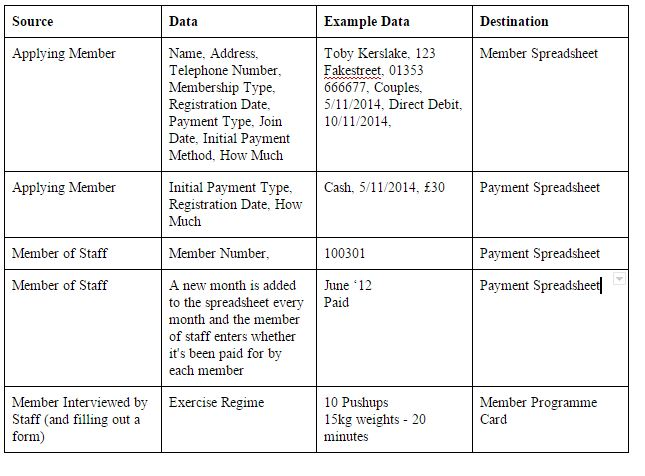
\includegraphics[width=\textwidth]{InvestigationTable1.JPG}
    \caption{Data Sources and Destinations for the current system} \label{fig:Current Destinations}
\end{figure}

\subsubsection{Algorithms}

Hierarchy Charts

Gym Sign Up Process
\begin{python}
1. Information is attained from the client
	1.1 My client gives a form to their client to be promptly filled out
	1.2 The client then hands the sheet back into reception 
	1.3 The information provided on this sheets then enter manually into an excel spreadsheet
	1.4 Do they have an exercise plan? Then the plan is created based on an interview  with the client while they fill out a form
2.Create Membership Card
	2.1 Make sure all necessary details are correct
	2.2 print Membership card 
\end{python}

Payment Process
\begin{python}
1. Client enters
2. Are they paying upfront?
2.1. Process their payment
2.2. Enter the appropriate information into the correct spreadsheet
2.3 Allow them into the facility
3. Have they payed by direct debit?
3.1. Check to see if the payment went through
3.2. If it did allow them into the facility
3.3 If the payment didnt go through then ask them to pay upfront and return to section 2
3.4 If they refuse to pay ask them to leave
\end{python}

Pseudocode


Gym Sign Up Process

\begin{python}

START

Function GetInfo:
	Client fills out form
	Hands form into gym owner
	Owner enters the information into an excel spreadsheet
	IF they have an exercise plan:
		Owner creates a plan based on an interview with client and new form and enters this into it’s
own spreadsheet
	Owner creates Membership Card
	Owner checks to make sure all the info is correct
	Owner prints membership card and gives it to the new member

GetInfo

END

\end{python}

Payment Process

\begin{python}
Start

Function ClientPayment:
	Client enters
	IF paying upfront:
		PayingUpFront
	IF paying by direct debit:
		PayingDirectDebit
	IF they refuse to pay:
		AskThemToLeave

Function PayingUpFront:
	Owner processes payment
	Process their payment
	Enter payment information into the appropriate spreadsheet
	Allow them into the facility

Function PayingDirectDebit:
	Check to see if the payment went through
	IF payment didn’t go through:
		IF they want to pay up front:
			PayingUpFront
		ELSE IF they refuse to pay:
			AskThemToLeave
	ELSE IF the payment did go through:
		Allow them into the facility

Function AskThemToLeave:
	Ask them to leave

ClientPayment 

END
\end{python}

Flow Charts

\begin{figure}[H]
    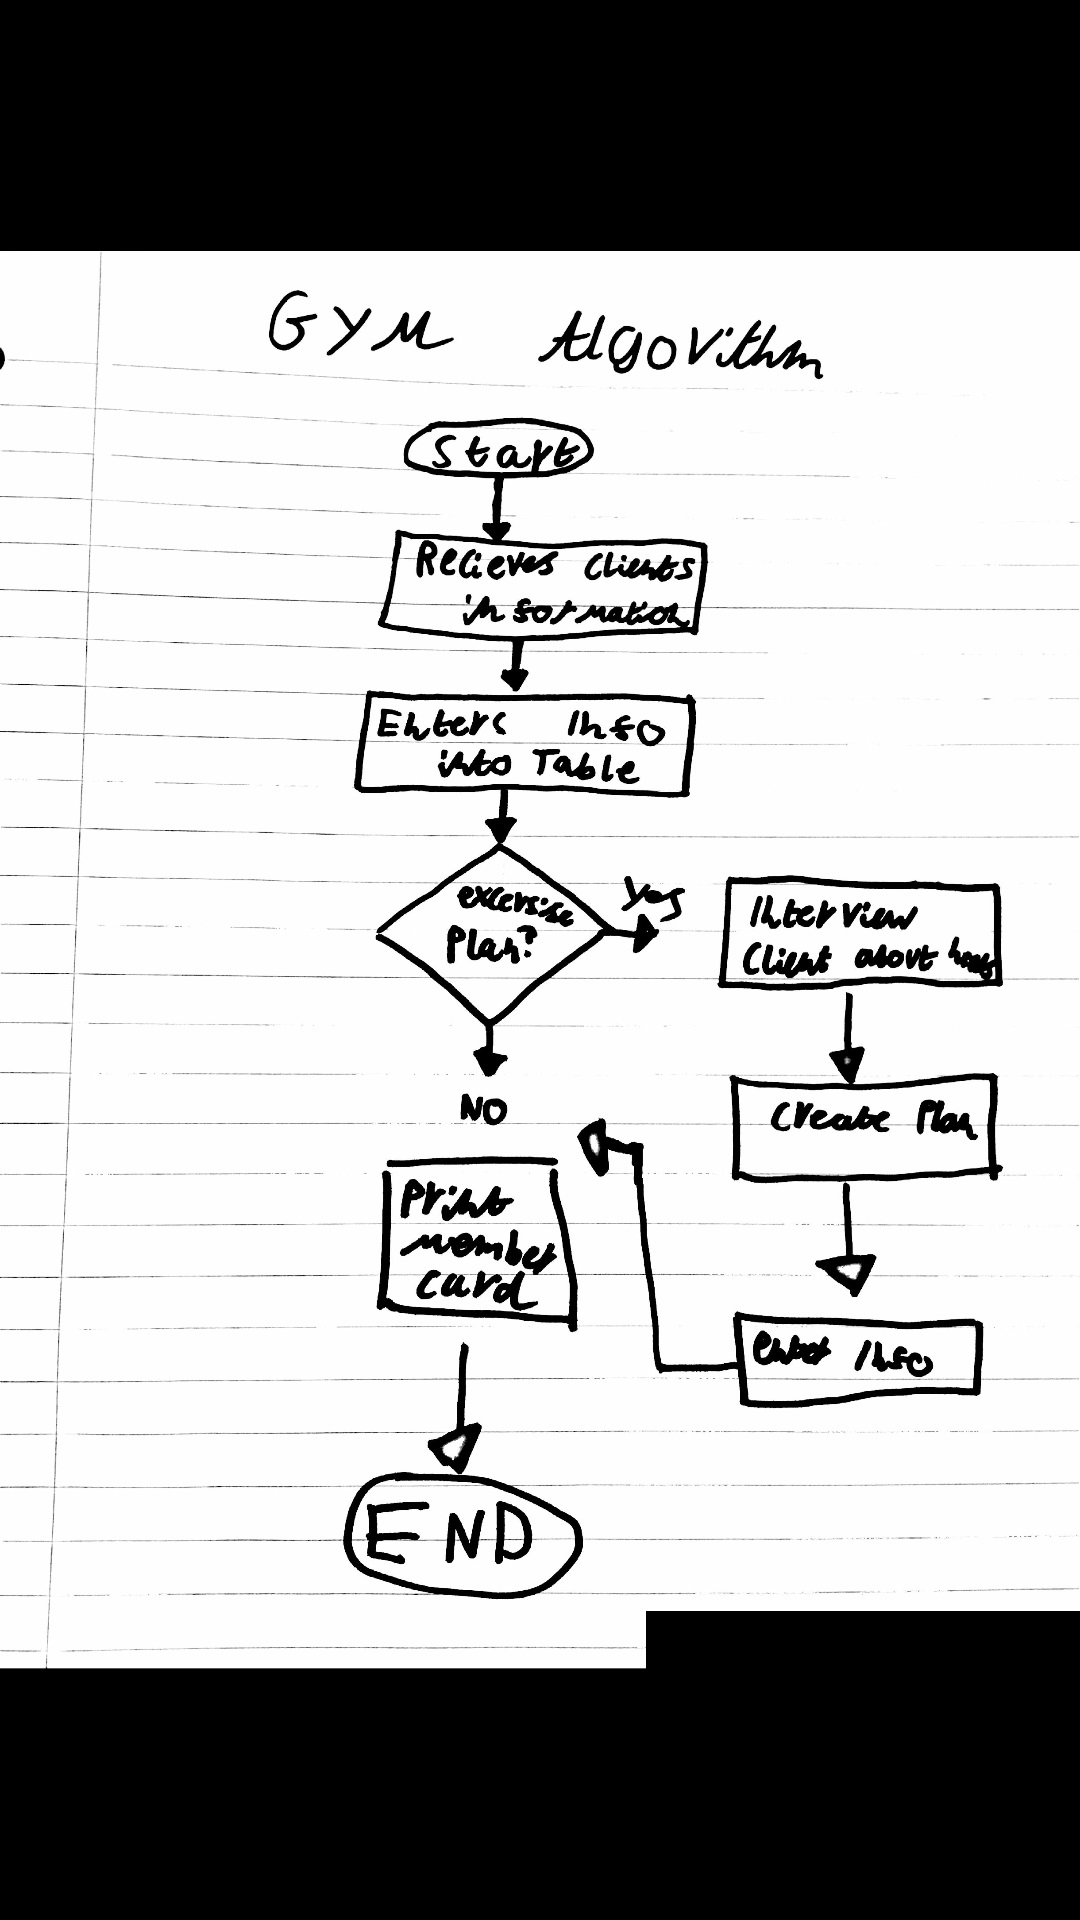
\includegraphics[width=\textwidth]{GymAlgorithm.jpg}
    \caption{Algorithm for the gym sign up process} \label{fig:Algorithm for the gym sign up process}
\end{figure}

\begin{figure}[H]
    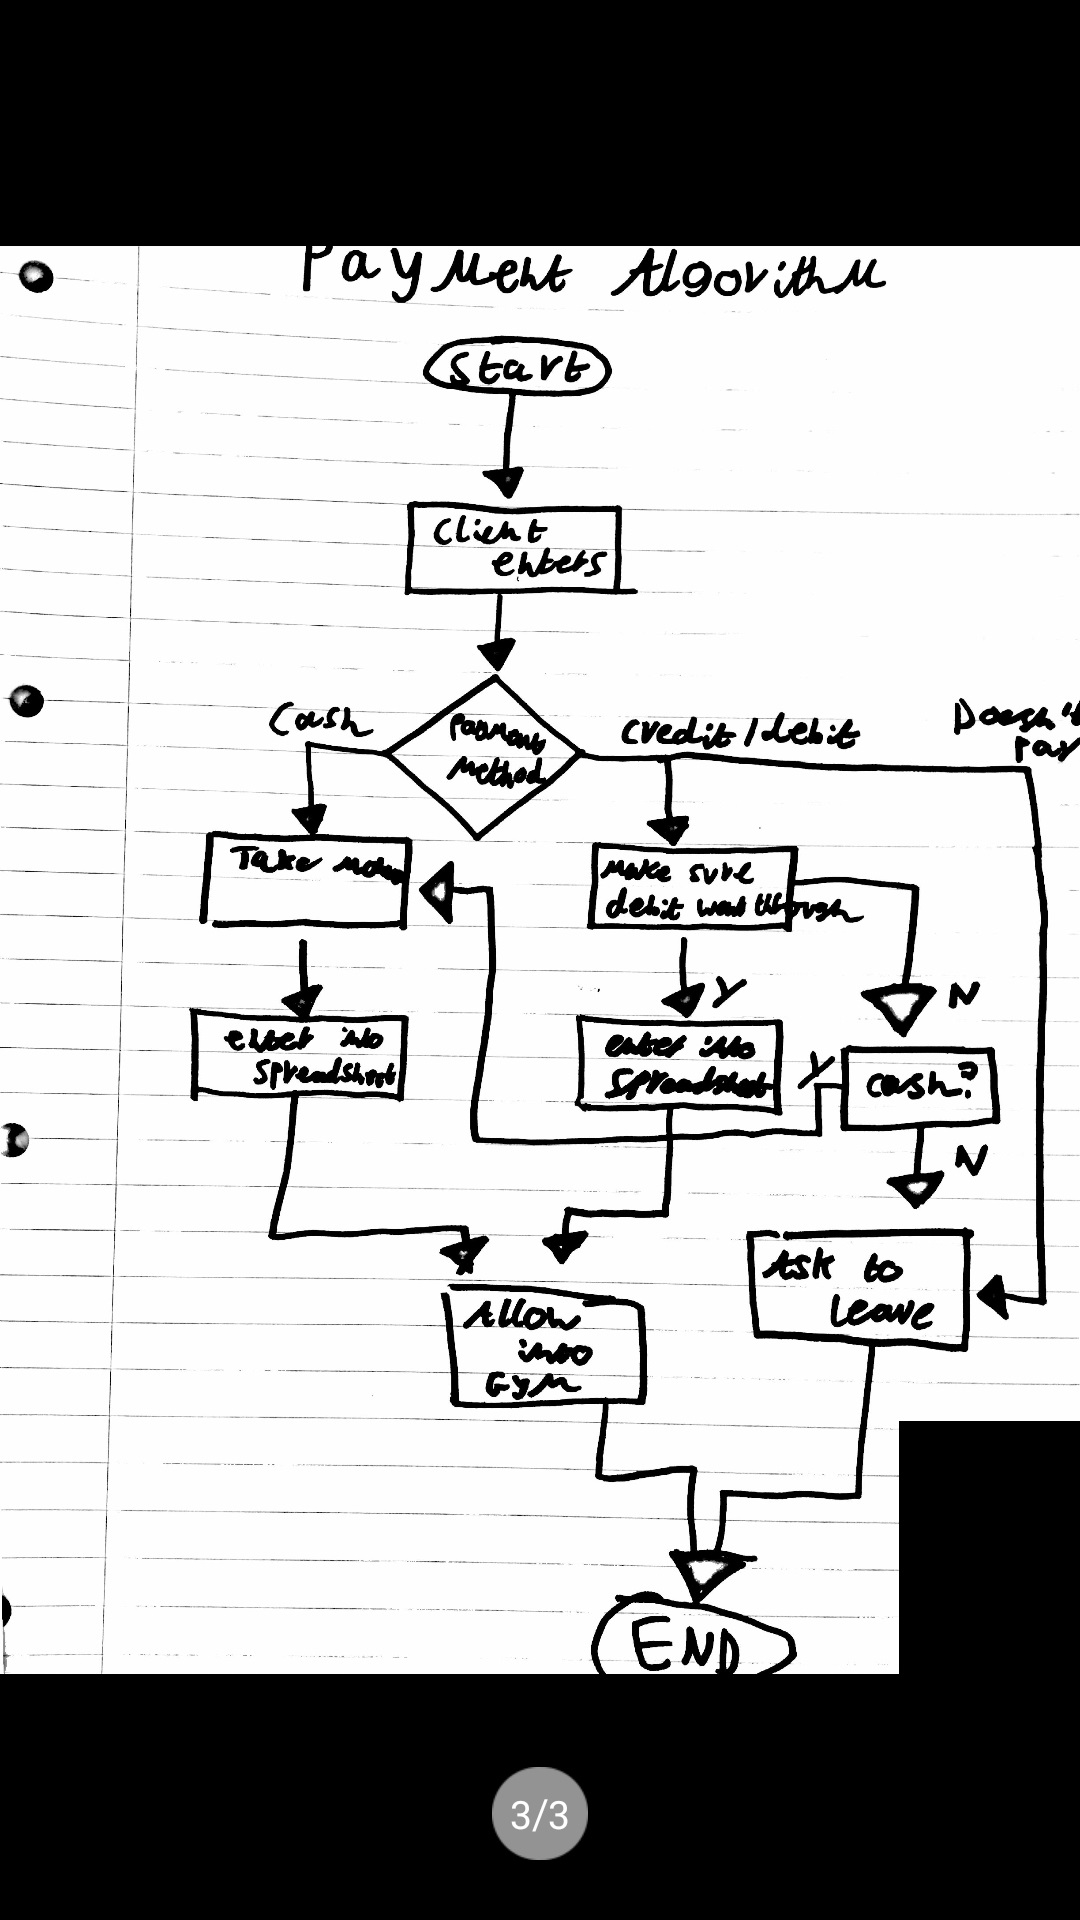
\includegraphics[width=\textwidth]{PaymentAlgorithm.jpg}
    \caption{Algorithm for the payment process} \label{fig:Algorithm for the payment process}
\end{figure}

\subsubsection{Data flow diagram}

\begin{figure}[H]
    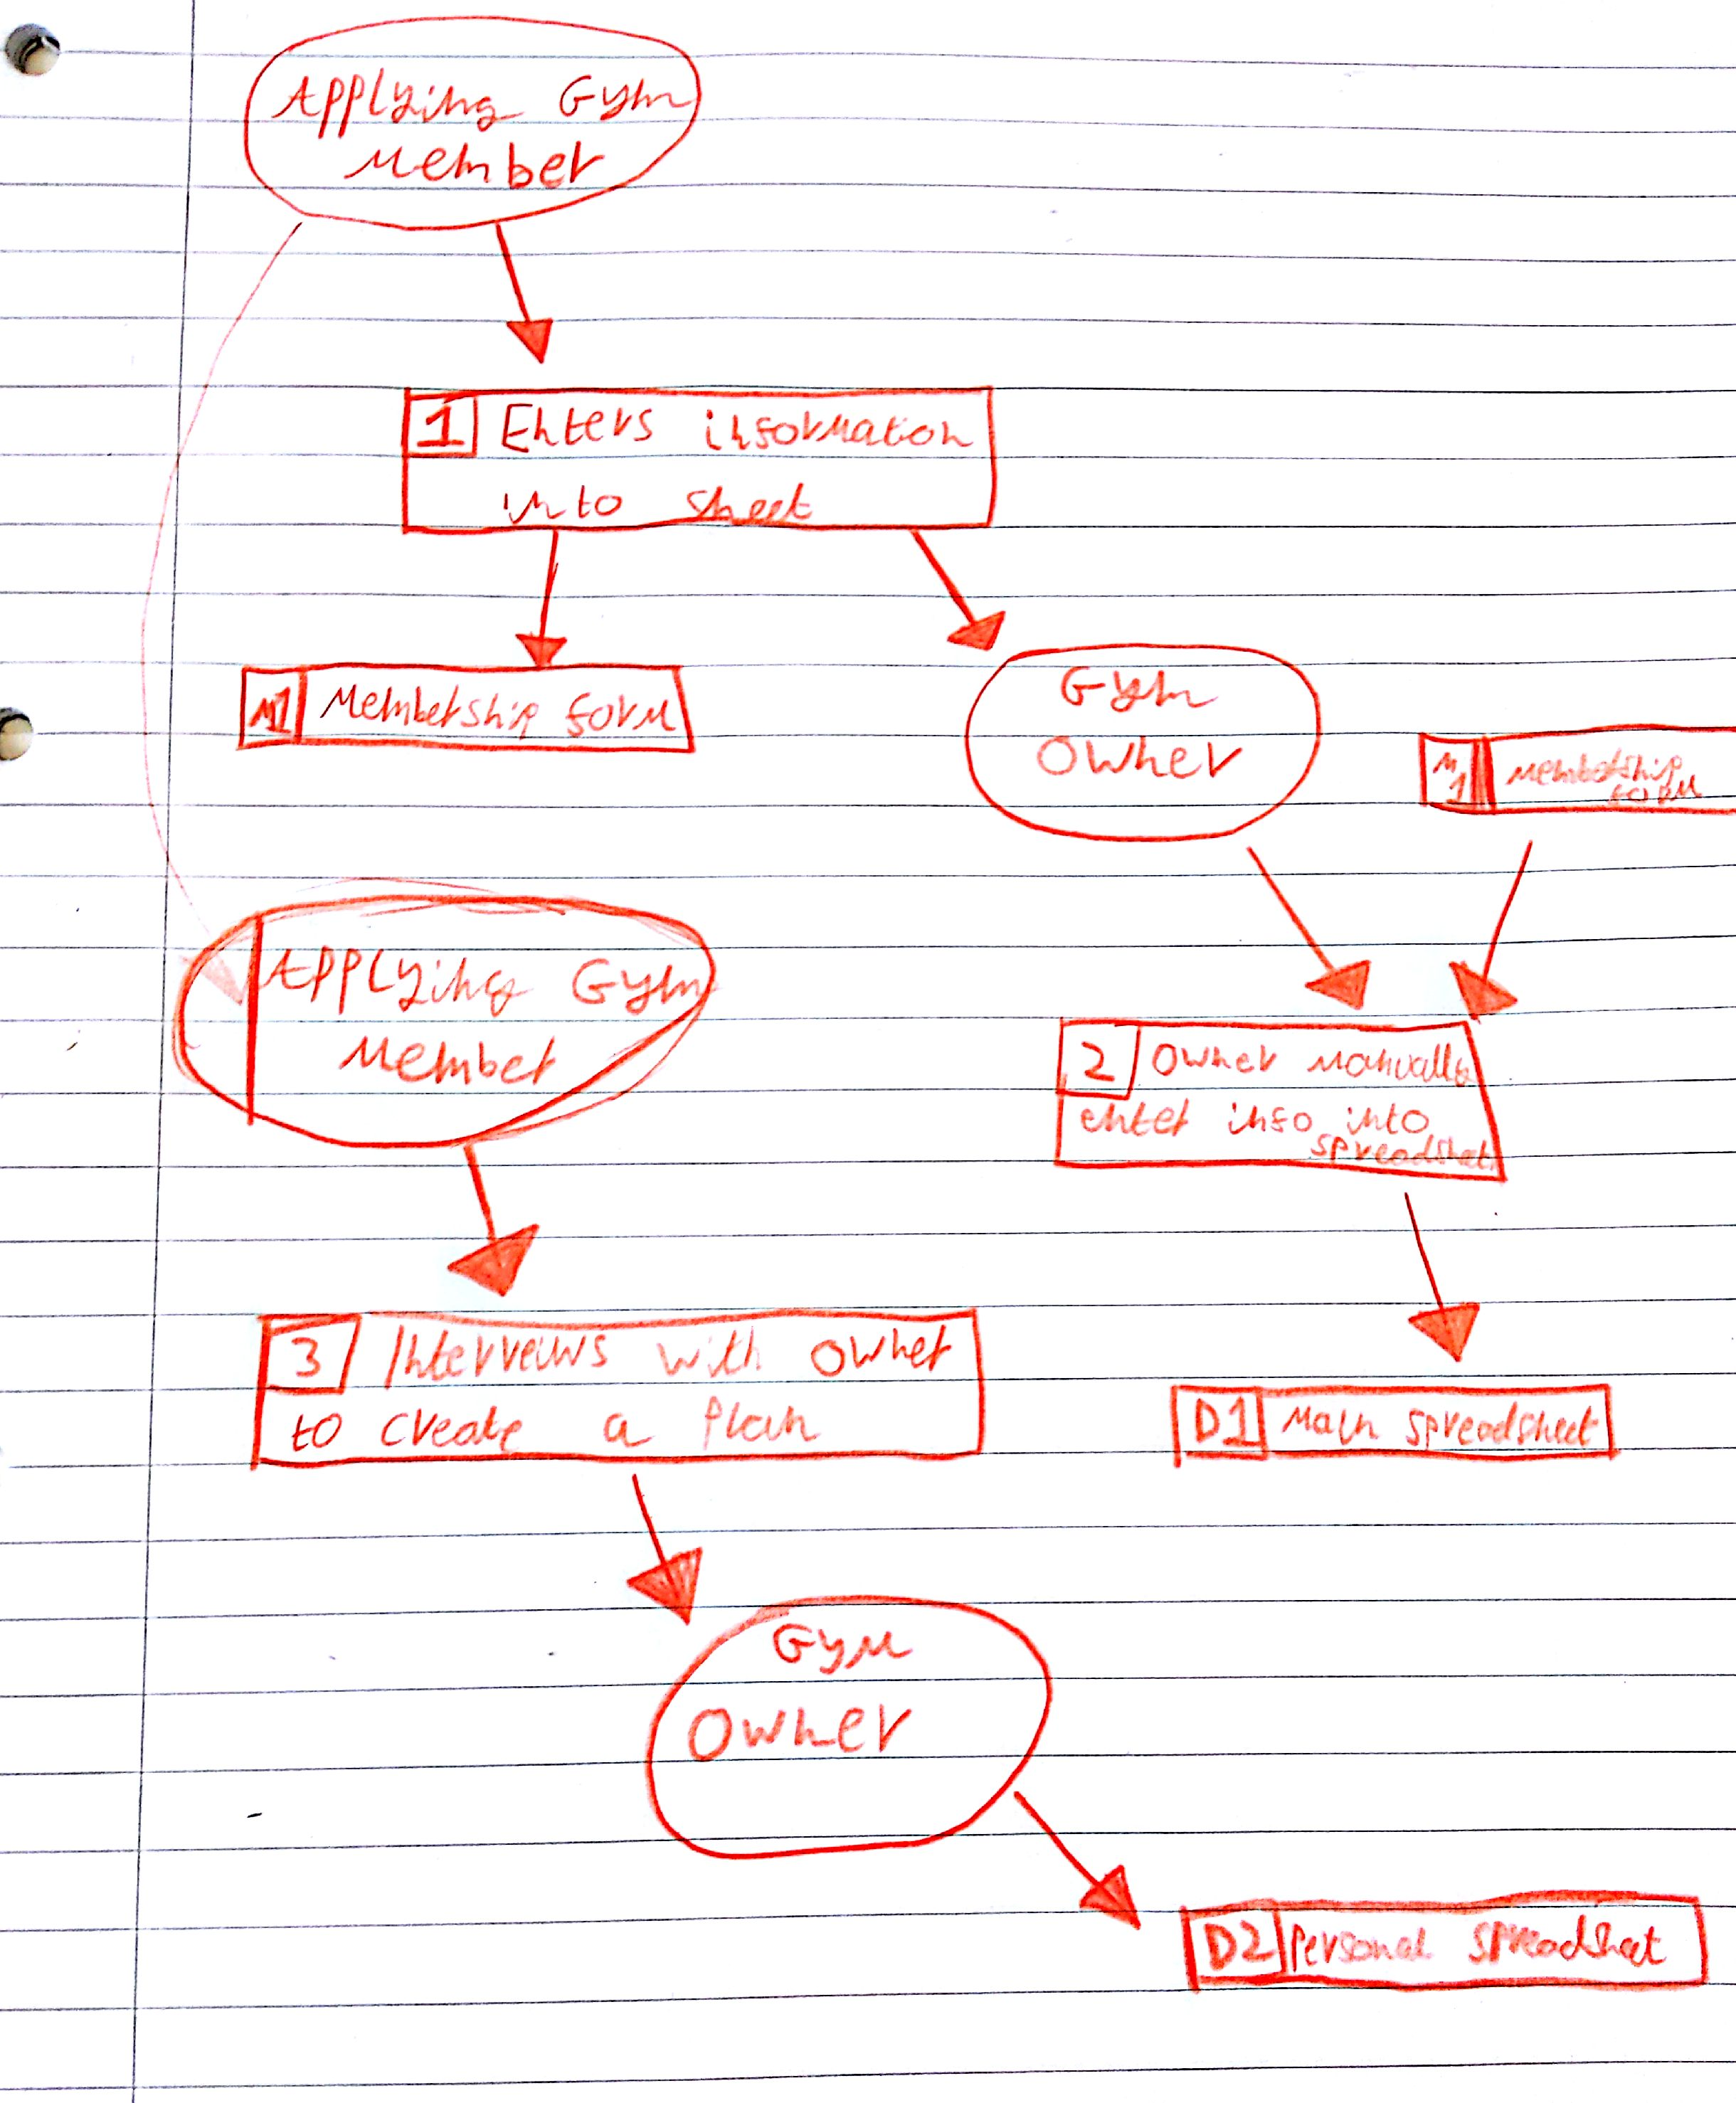
\includegraphics[width=\textwidth]{DFD-Current.jpg}
    \caption{Data Flow Diagram For The Current System} \label{fig:Data Flow Diagram For The Current System}
\end{figure}


\subsubsection{Input Forms, Output Forms, Report Formats}

\begin{figure}[H]
    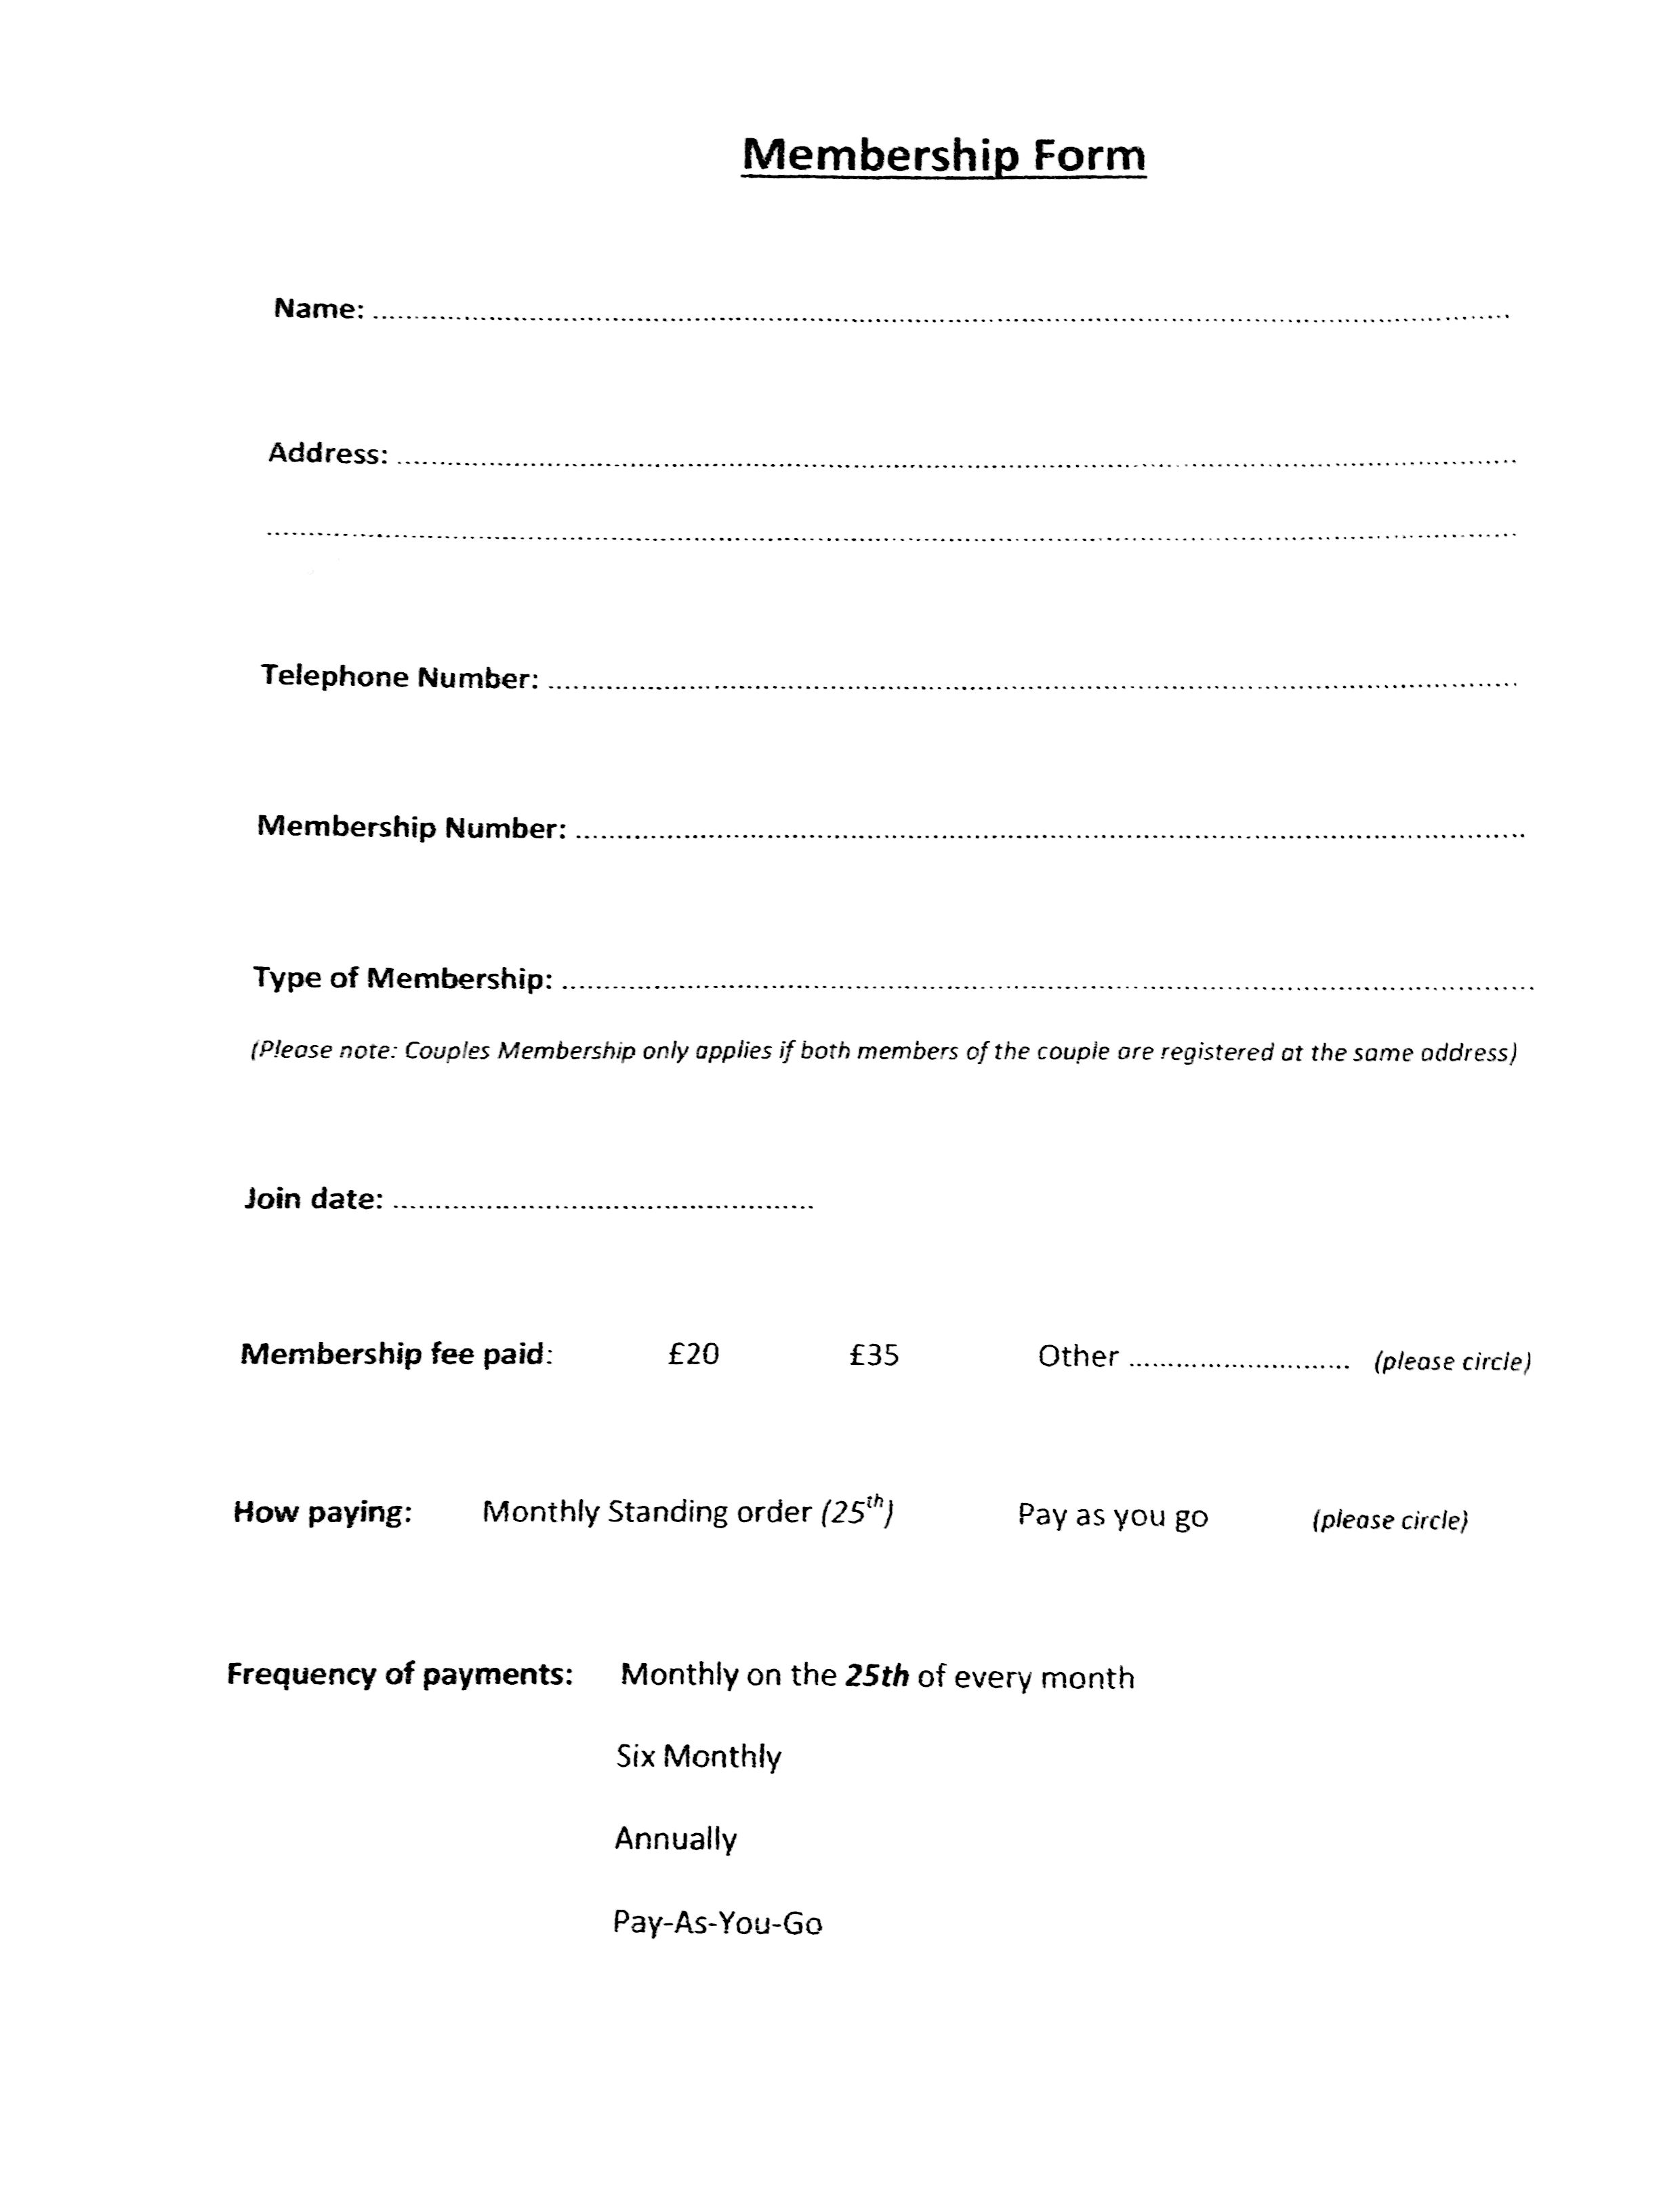
\includegraphics[width=\textwidth]{MembershipForm.jpg}
    \caption{This is the Membership Sign up form. This is printed and handed to applying members upon sign up and can either be filled out at the premises or filled out elsewhere and handed back in to reception. It is used to gather basic information for the membership and payment details spreadsheets.} \label{fig:Membership Sign up Form}
\end{figure}

\begin{figure}[H]
    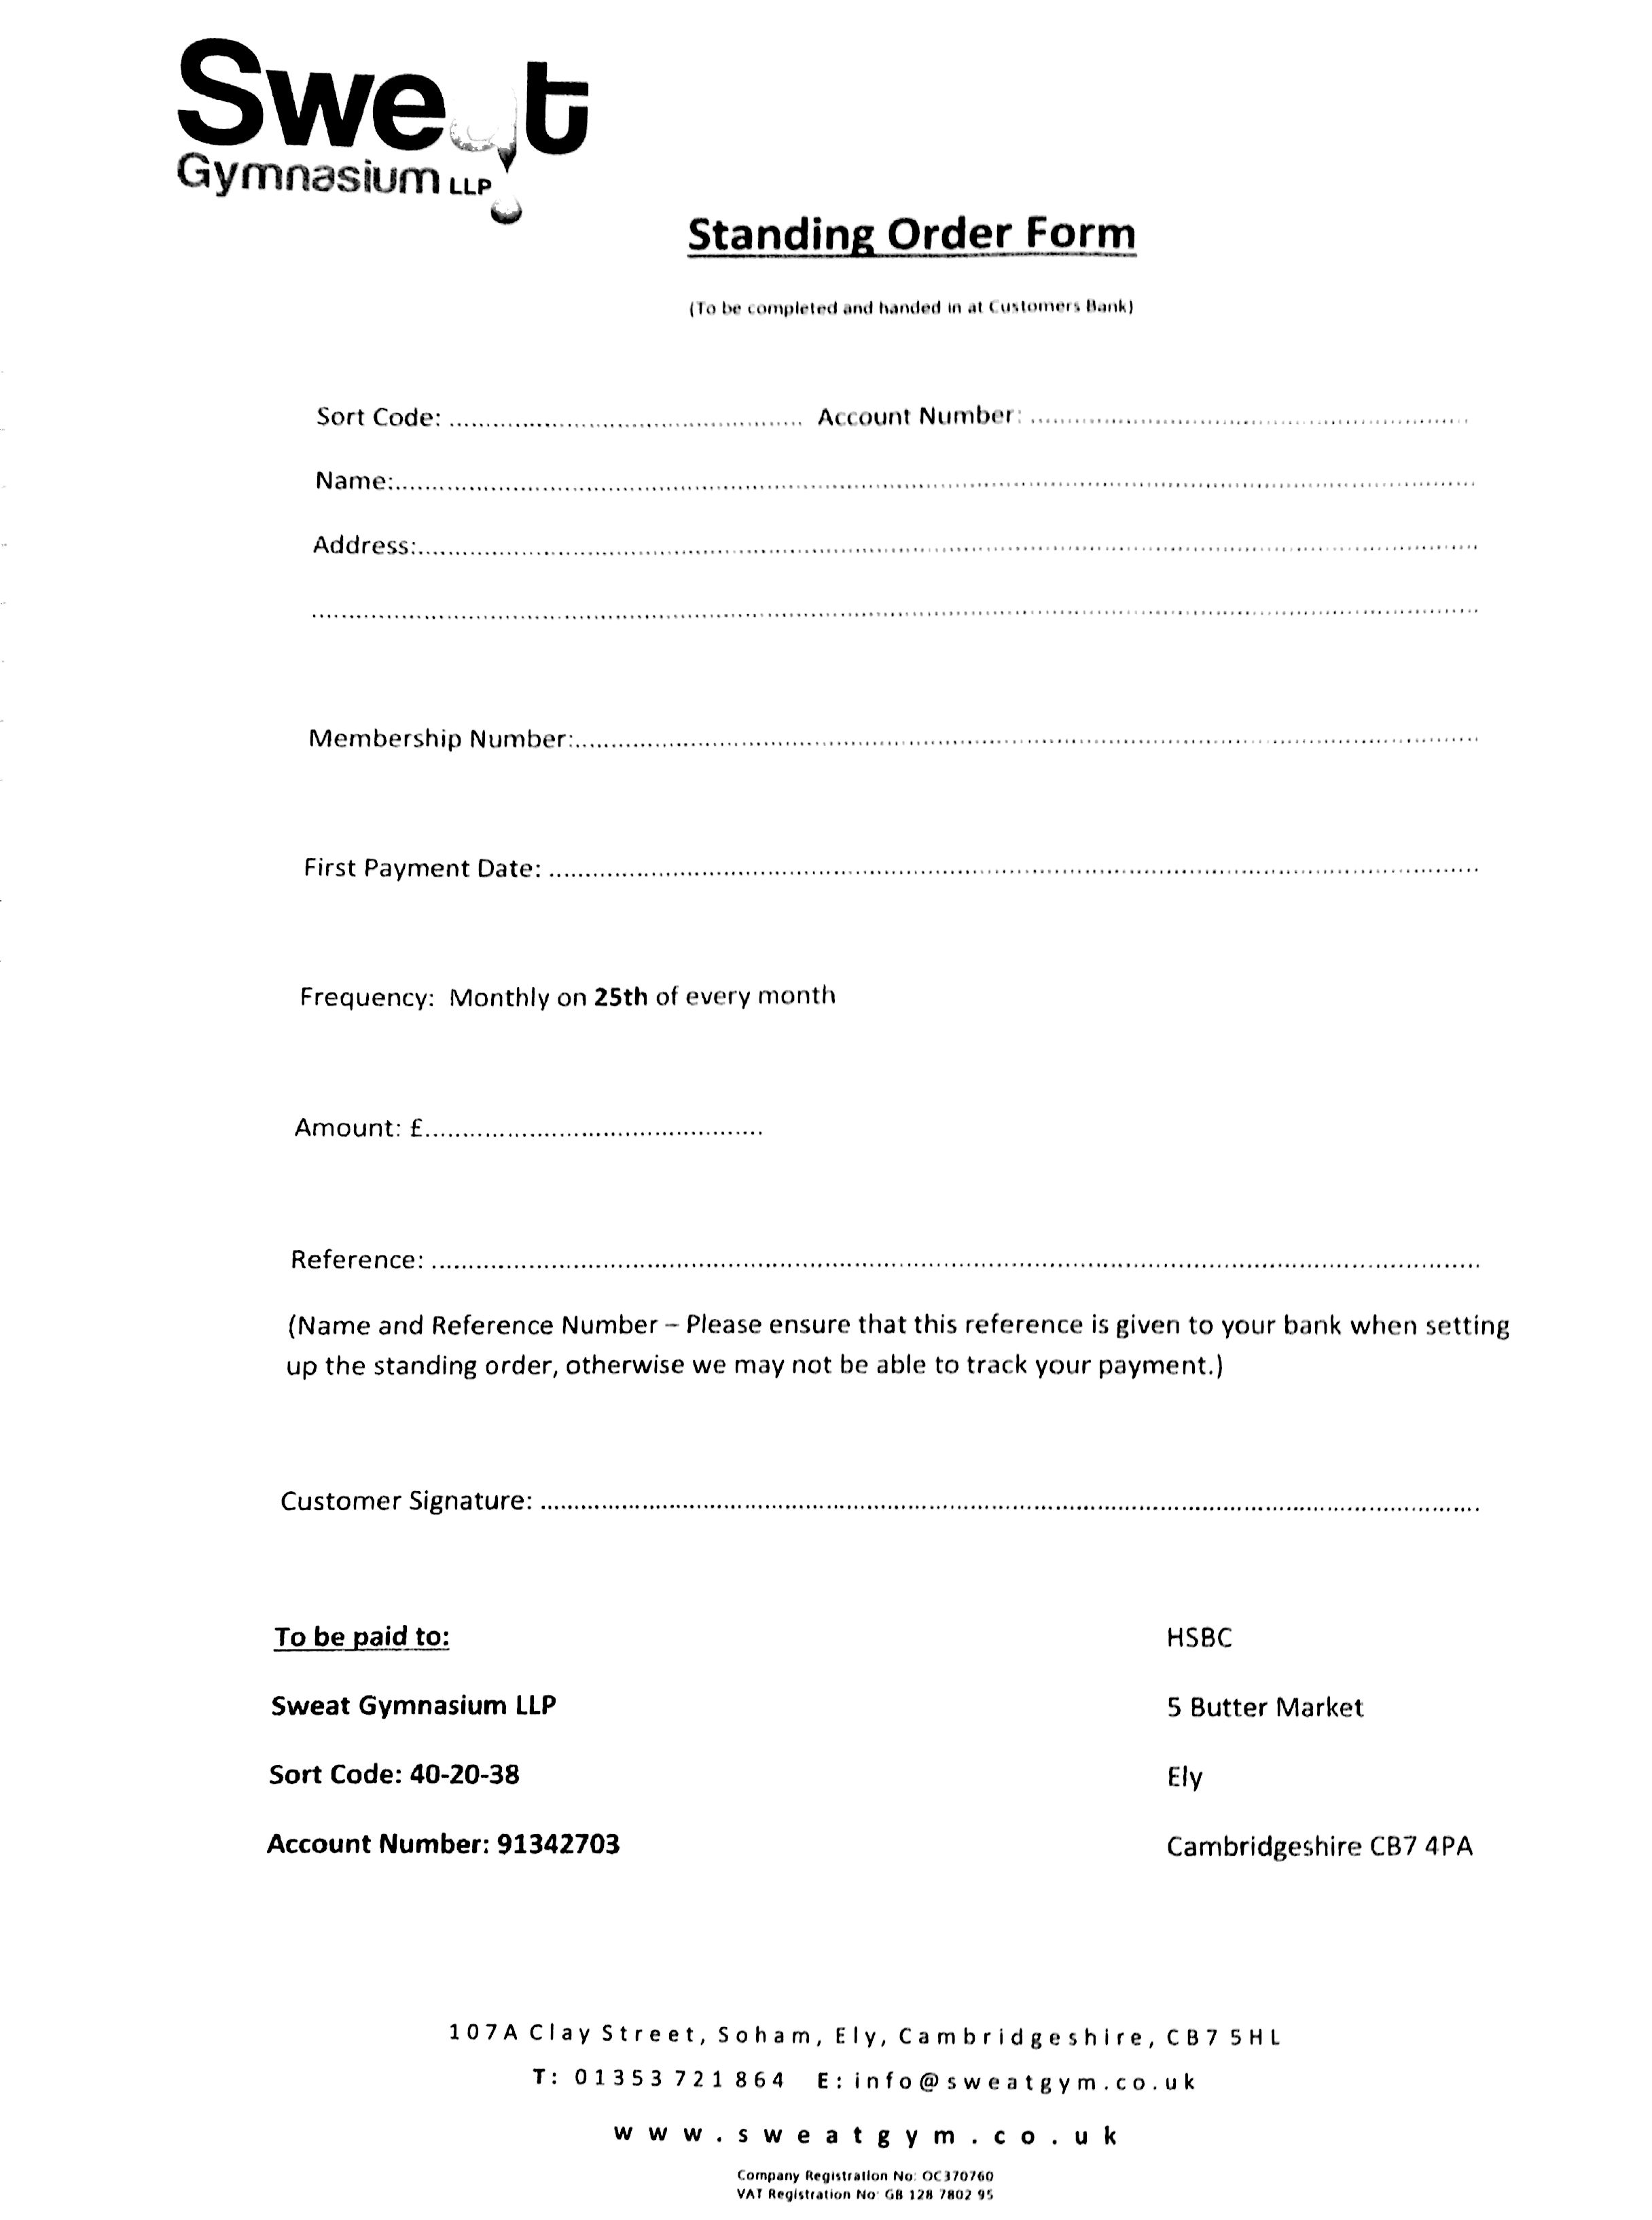
\includegraphics[width=\textwidth]{StandingOrderForm,jpeg.jpg}
    \caption{This is the Standing Order Form. This is printed and handed to the user along with the membership form and is for the member to fill in and hand to their bank so they make the correct payment. Some of this form can be filled in with assistance from a member of staff. For example their membership number.} \label{fig:Standing Order Form }
\end{figure}

\begin{figure}[H]
    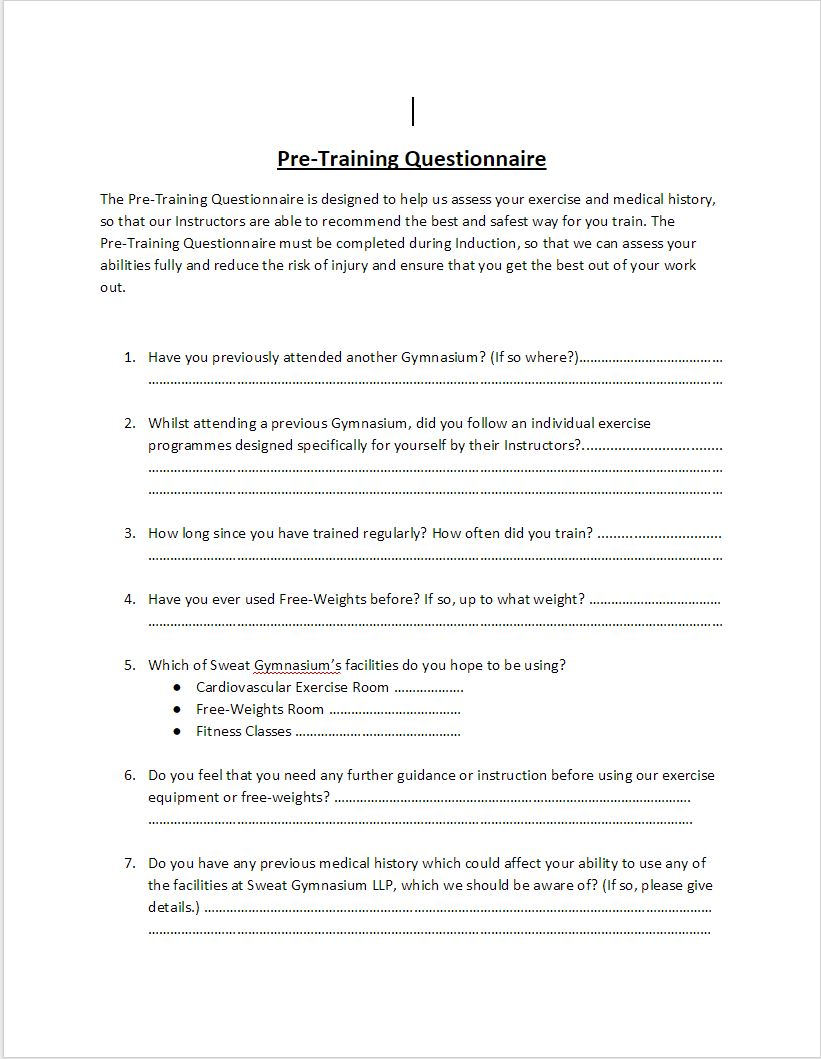
\includegraphics[width=\textwidth]{RegimeInterveiw1.JPG}
    \caption{Regime Interveiw Part 1} \label{fig:Regime Interveiw Part 1}
\end{figure}

\begin{figure}[H]
    
\includegraphics[width=\textwidth]{RegimeInterveiw2.JPG}
    \caption{Regime Interveiw Part 2. The regime interview/Pre-Training Questionaire is filled out by the applying gym member and a member of staff to determine what the members regime should appropriately consist of. This information is compiled into different exercises and routines stored on the members programme card shown in the next figure. Afterwards these sheets are disposed of. } \label{fig:Regime Interveiw Part 2}
\end{figure}

\begin{figure}[H]
    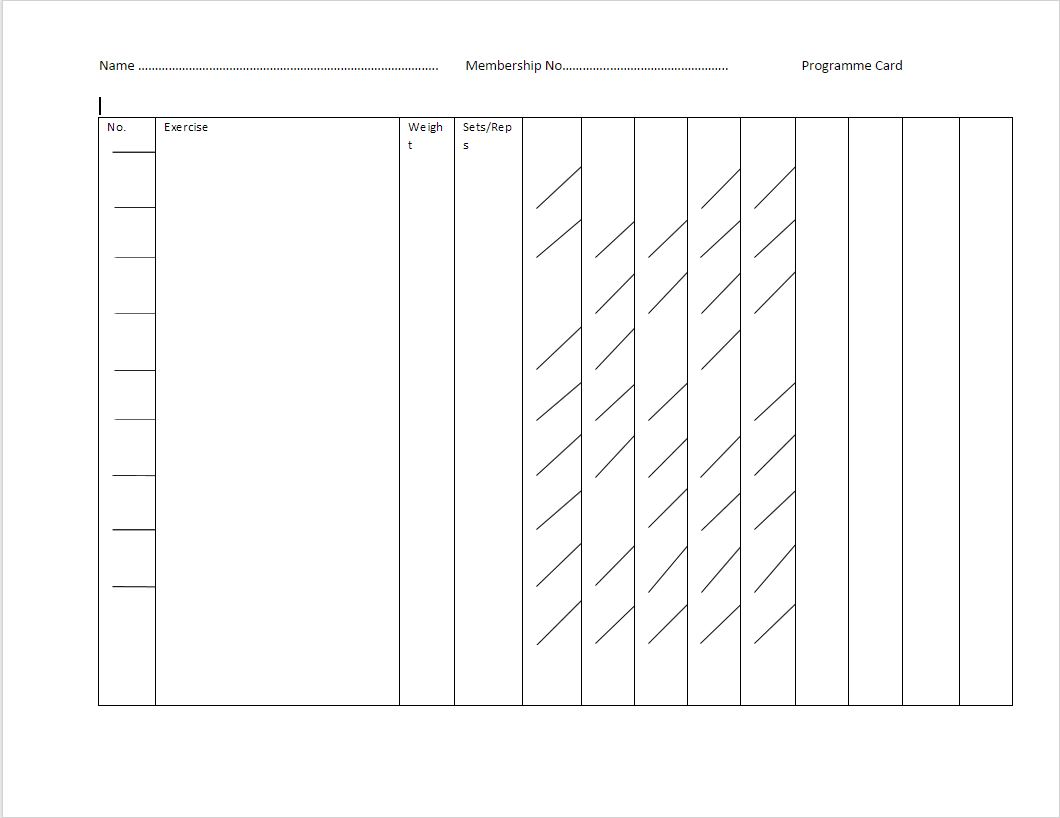
\includegraphics[width=\textwidth]{Programmecard.JPG}
    \caption{The Programme Card is where a Gym members personal regime is written down and organised, with 2 columns to determine the number of reps/weights involved with the exercise. The other columns that contain slashes have no purpose and are just there to fill space. This shows the forms poor design and thus it will probably have to be redisigned for use with the new system.} \label{fig:Programme Card}
\end{figure}

\begin{figure}[H]
    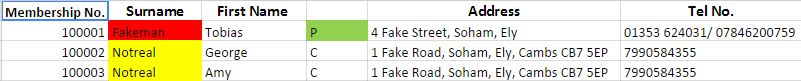
\includegraphics[width=\textwidth]{MembershipSpreadsheet1.JPG}
    \caption{Member Details Spreadsheet Part 1} \label{fig:Member Details Spreadsheet Part 1}
\end{figure}

\begin{figure}[H]
    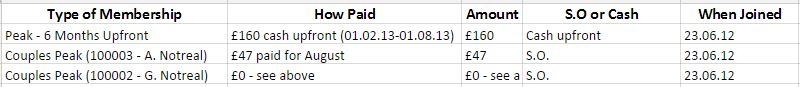
\includegraphics[width=\textwidth]{MembershipSpreadsheet2.JPG}
    \caption{Member Details Spreadsheet Part 2} \label{fig:Member Details Spreadsheet Part 2}
\end{figure}

\begin{figure}[H]
    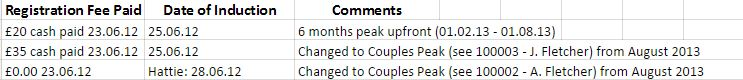
\includegraphics[width=\textwidth]{MembershipSpreadsheet3.JPG}
    \caption{Member Details Spreadsheet Part 3. All the information stored in this spreadsheet was gathered from previous forms or noted down by a member of staff during the members induction and then entered into the spreadsheet. This is stored locally on a workstation in the gym where only authorised users can gain access to it. The spreadsheets are rarely printed out except in special circumstances like accounting purposes.} \label{fig:Member Details Spreadsheet Part 3}
\end{figure}

\begin{figure}[H]
    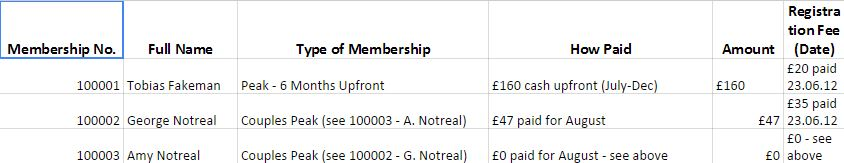
\includegraphics[width=\textwidth]{PaymentSpreadsheet1.JPG}
    \caption{Payment Details Spreadsheet part 1} \label{fig:Payment Details Spreadsheet Part 1}
\end{figure}

\begin{figure}[H]
    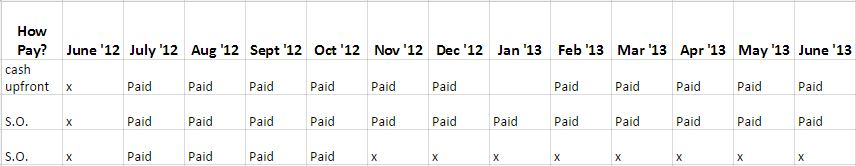
\includegraphics[width=\textwidth]{PaymentSpreadsheet2.JPG}
    \caption{Payment Details Spreadsheet part 2. This spreadsheet contains payment details collected from the previous forms and during the induction period. It also keeps track of every month and whether the member has paid for said month.  } \label{fig:Payment Details Spreadsheet part 2 }
\end{figure}


\subsection{The proposed system}

My proposed system uses a database to keep track of all the data that my client previously kept in an excel spreadsheet using a program created in the python programming language using the PyQt 4 library. This is because its the language I'm most comfortable with and allows for the creation of intuitive UI and the creation of an executable program using the software cx freeze ensuring that the system will be easily usable by my client.

\subsubsection{Data sources and destinations}

\begin{figure}[H]
    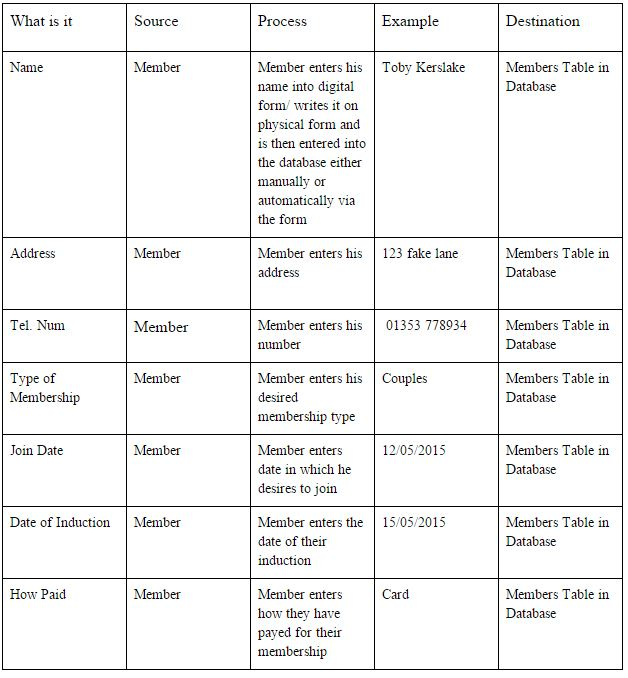
\includegraphics[width=\textwidth]{Data Sources and Definitions - Proposed 2.JPG}
    \caption{Data Sources and Destinations} \label{fig: Data Sources and Destinations }
\end{figure}

\begin{figure}[H]
    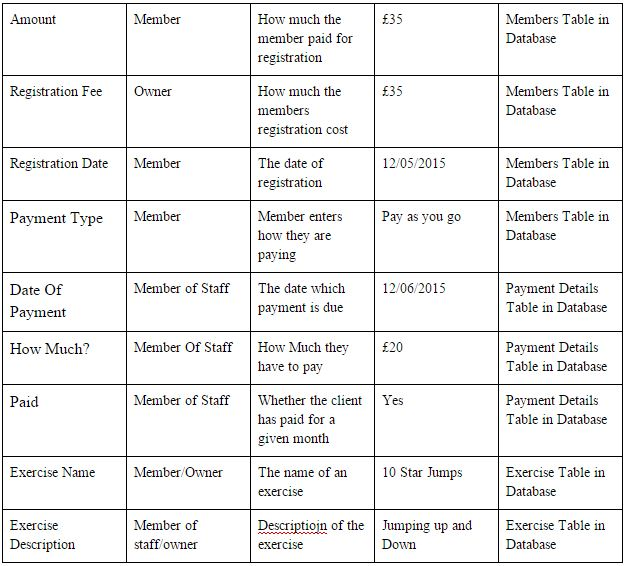
\includegraphics[width=\textwidth]{Data Sources and Definitions - Proposed.JPG}
    \caption{Data Sources and Destinations 2} \label{fig: Data Sources and Destinations 2 }
\end{figure}

\begin{figure}[H]
    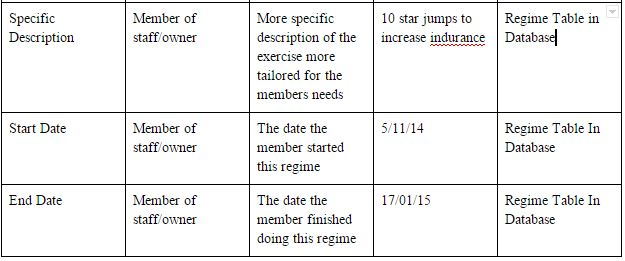
\includegraphics[width=\textwidth]{New Proposed Sources 3.JPG}
    \caption{Data Sources and Destinations 3} \label{fig: Data Sources and Destinations 3 }
\end{figure}

\subsubsection{Data flow diagram}

\begin{figure}[H]
    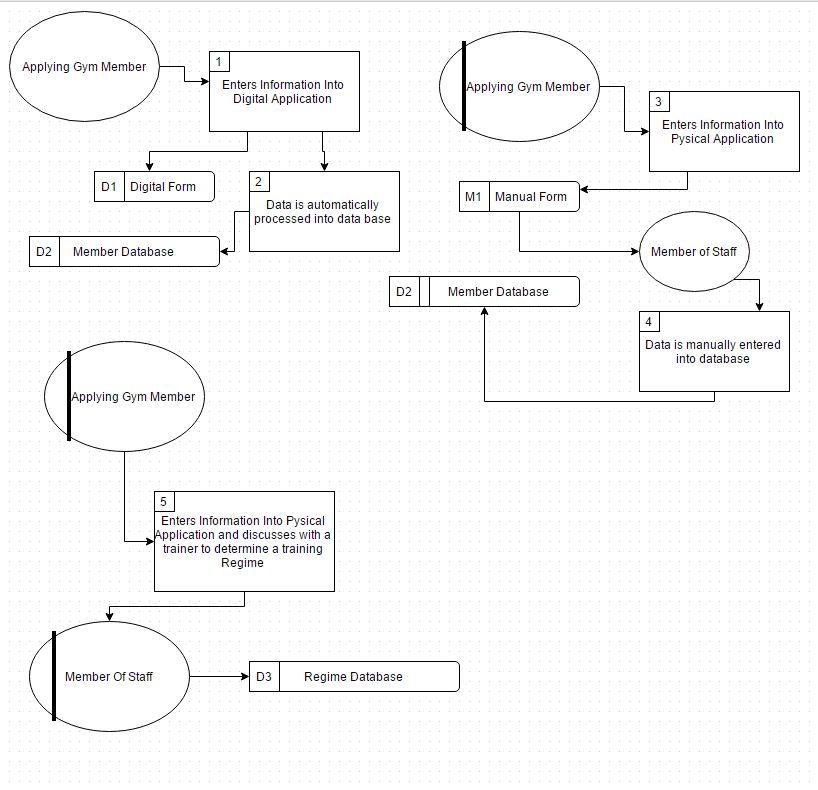
\includegraphics[width=\textwidth]{ProposedDFD.JPG}
    \caption{Data Flow Diagram} \label{fig: Data Flow Diagram }
\end{figure}

\begin{figure}[H]
    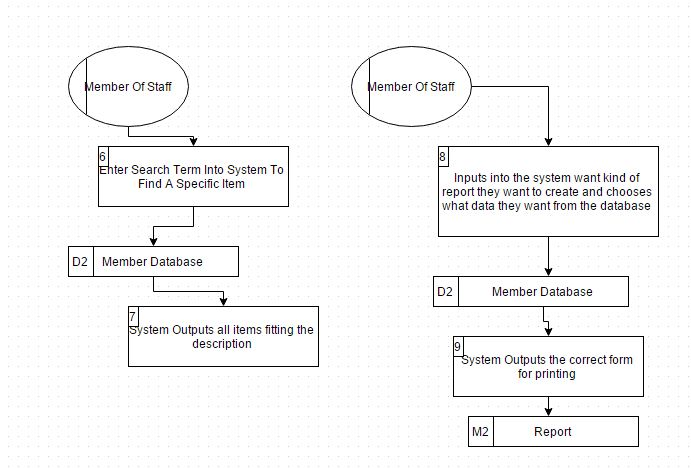
\includegraphics[width=\textwidth]{dfd_2.JPG}
    \caption{Data Flow Diagram} \label{fig: Data Flow Diagram }
\end{figure}

\subsubsection{Data dictionary}

\begin{figure}[H]
    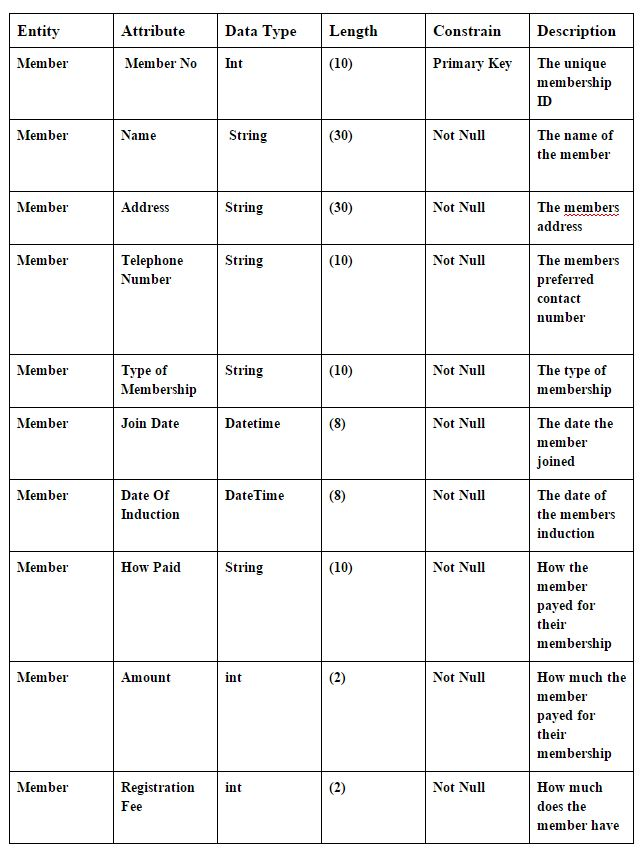
\includegraphics[width=\textwidth]{DataDictionaryProposed.JPG}
    \caption{Data Dictionary} \label{fig: Data Destinations and Sources }
\end{figure}

\begin{figure}[H]
    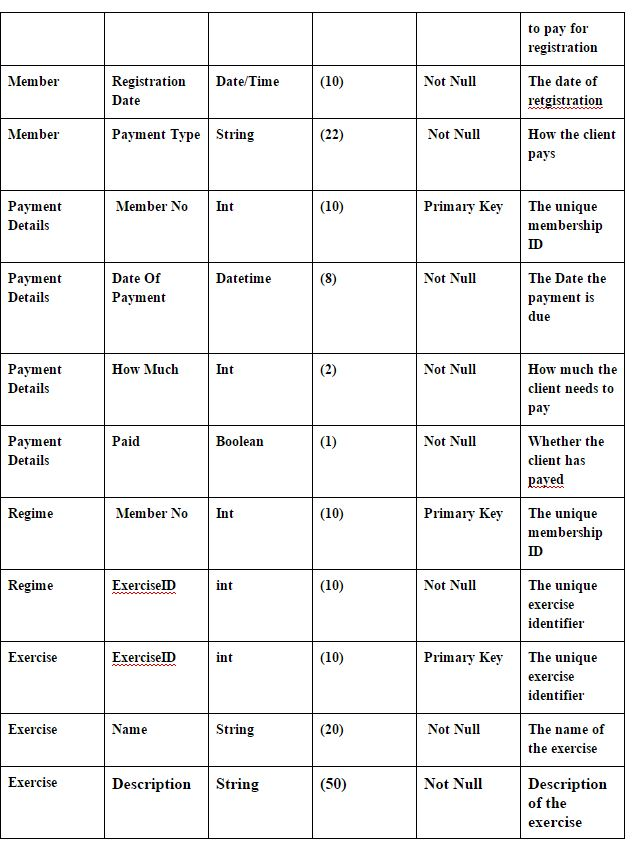
\includegraphics[width=\textwidth]{DataDictionaryProposed2.JPG}
    \caption{Data Dictionary 2} \label{fig: Data Destinations and Sources 2 }
\end{figure}

\begin{figure}[H]
    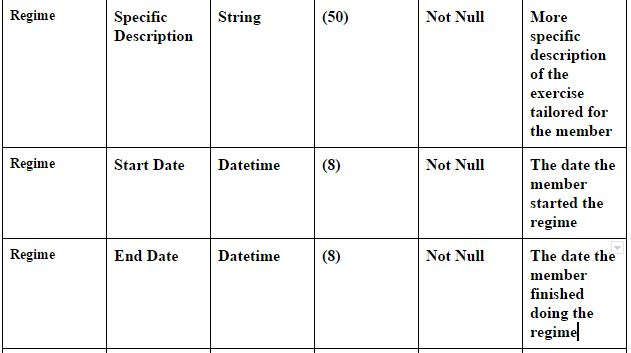
\includegraphics[width=\textwidth]{New_dictionary3.JPG}
    \caption{Data Dictionary 3} \label{fig: Data Destinations and Sources 2 }
\end{figure}

\subsubsection{Volumetrics}

I have decided on an initial size of 2000 members since the gym is nearing that number of members and will inevitably achieve this amount of clients.  My client has said the amount of clients he gains isn't consistent as people often register in different sized groups. Although over the past year he has gained 560 new members and roughly 400 members the year before, and the year before that. This means that we can estimate that in about a year and a half the gym will exceed 2000 members. The size of the database can be increased at a later date when needed.  

Each member has 11 - 16 fields of data in total, with each data field taking up 1 KB of data.

16 * 1KB * 2000 = 32000 KB
32000 / 1024 = 31.25 MB

The rest of the system should take up a small amount of space that will probably take up about 3MB.

31.25 MB + 3MB = 34.25 MB

\section{Objectives}

\subsection{General Objectives}

    \begin{itemize}  

        \item Clear/easy to understand layout structure for member/client records viewing/observation 

        \item Clear/easy to understand layout structure for all member/client data input  

        \item Clear/easy to understand layout for creating and printing invoices/ member records
        
        \item Clear/easy to understand digital/physical input forms for users to enter data
        
        \item Secure system thats password protected so that only appropriate staff members can use the system
        
        \item Cerain options like deleting items from the database restricted to only an administrator/ sepearte password that only higher level staff members can access
        
        \item Presentable, minimalistic GUI that can be easily understood and interacted with by the users 
        
        \item Appropriate Screen outputs for example dialog boxes and the presentation of the database presented in the GUI mockup.

    \end{itemize}

\subsection{Specific Objectives}

Client/Member Record Viewing/Data Input

\begin{itemize}  

        \item Easy to use Simple Gui with clearly labelled buttons to choose an option (as shown in the mock-ups I presented my client).
        \item Their should be buttons for opening a table, add to it, editing it, deleting an item, creating an invoice or physical record, and searching for something specific.
        \item Each of these buttons should open up either drop down menus or entirely new windows, depending on which is more user friendly, and display further options within those commands.
        \item The interface for entering new information should be easy to use and clearly labelled for adding each attribute to the specified table.
        \item Their should be an easy/ifficient way to switch and search between all of the tables in the database.
        \item the .db file made in SQL should be password protected so it can't just be opened in another program without being crredible enough to know the password.
        \item Avoid more novice users accidentally deleteing items by having a secondary password for higher level access.
        \item Store backups of the database online using a system like dropbox or GitHub so that in the event of data corruption there would be recent version to backup to
        \item Storing the latest version of the spreasheet locally also adds an extra layer of security as the most recent version wont be easily accessable exept by people with direct access to the workstation.
    \end{itemize}


System Outputs

\begin{itemize}  

        \item Easy to create reports containing all of a specific clients information in an organised manner on as little paper as legibly possible.
        \item Easy to create invoices for members based off of the information stored in the tables.
        \item Reports should include Invoices, database table printouts, member reports giving details selected from the databases.
        \item These reports should be printable so that they can be given to members and stored physically
        
\end{itemize}

Input Forms

    \begin{itemize}  

        \item Easy to fill out digital input forms, maybe made in HTML that can be distributed by email or through the gyms website that the program could automatically search for a recieve when being opened.
        \item Printable versions off these forms that can be created to be filled out by hand by less technically inclined clients that can then have their information manually entered into the system by a member of staff.

    \end{itemize}

\subsection{Core Objectives}

\begin{itemize}
        \item Easy to use Simple Gui with clearly labelled buttons to choose an option (as shown in the mock-ups I presented my client).
        \item Their should be buttons for opening a table, add to it, editing it, deleting an item, creating an invoice or physical record, and searching for something specific.
        \item Each of these buttons should open up either drop down menus or entirely new windows, depending on which is more user friendly, and display further options within those commands.
        \item The interface for entering new information should be easy to use and clearly labelled for adding each attribute to the specified table.
        \item Their should be an easy/ifficient way to switch and search between all of the tables in the database.
        \item the .db file made in SQL should be password protected so it can't just be opened in another program without being crredible enough to know the password.
        \item Avoid more novice users accidentally deleteing items by having a secondary password for higher level access.
        \item Store backups of the database online using a system like dropbox or GitHub so that in the event of data corruption there would be recent version to backup to
        \item Storing the latest version of the spreasheet locally also adds an extra layer of security as the most recent version wont be easily accessable exept by people with direct access to the workstation.
                \item Easy to create reports containing all of a specific clients information in an organised manner on as little paper as legibly possible.
        \item Easy to create invoices for members based off of the information stored in the tables.
        \item Reports should include Invoices, database table printouts, member reports giving details selected from the databases.
        \item These reports should be printable so that they can be given to members and stored physically
        

\end{itemize}


\subsection{Other Objectives}

\begin{itemize}
     \item Easy to fill out digital input forms, maybe made in HTML that can be distributed by email or through the gyms website that the program could automatically search for a recieve when being opened.
        \item Printable versions off these forms that can be created to be filled out by hand by less technically inclined clients that can then have their information manually entered into the system by a member of staff.
        
\end{itemize}

\section{ER Diagrams and Descriptions}


\subsection{ER Diagram}

\begin{figure}[H]
    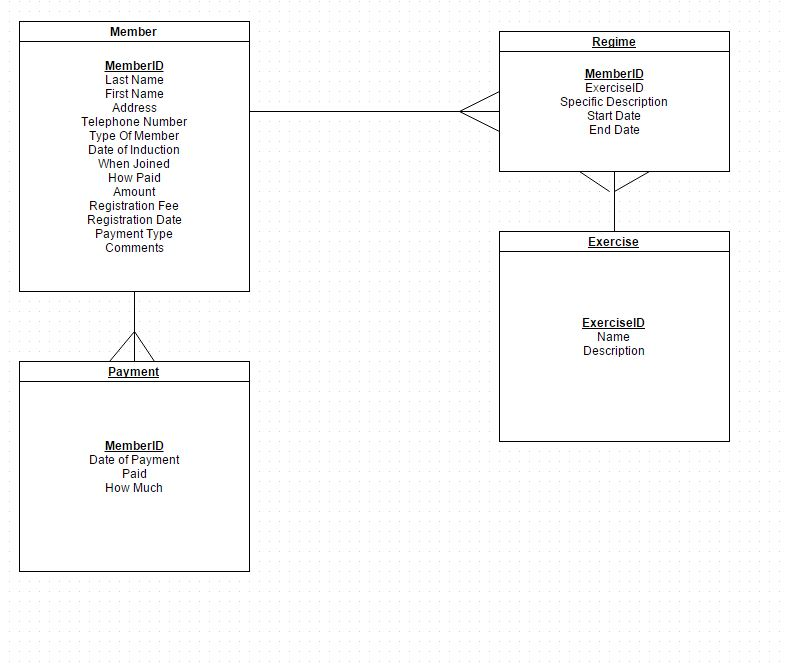
\includegraphics[width=\textwidth]{-ERDiagram.JPG}
    \caption{ER Diagram} \label{fig: ER Diagram}
\end{figure}


\subsection{Entity Descriptions}

Membership Details(\textbf{\underline{Membership No.}}, Last Name, First Name, Address, Telephone No., Type Of Membership, Date of Induction, When Joined, How Paid,amount, registration fee, Registration Date, Payment Type, Comments)

Payment Details(\textbf{\underline{Membership No.}},Date of Payment, How Much, Paid)

Regime(\textbf{\underline{Membership No.}},ExerciseID,Specific Description, Start Date, End Date)

Exercise(\textbf{\underline{ExerciseID}}, Name, Description)

\section{Object Analysis}

\subsection{Object Listing}

Membership Details

Payment Details

Regime

Exercise

\subsection{Relationship diagrams}

\begin{figure}[H]
    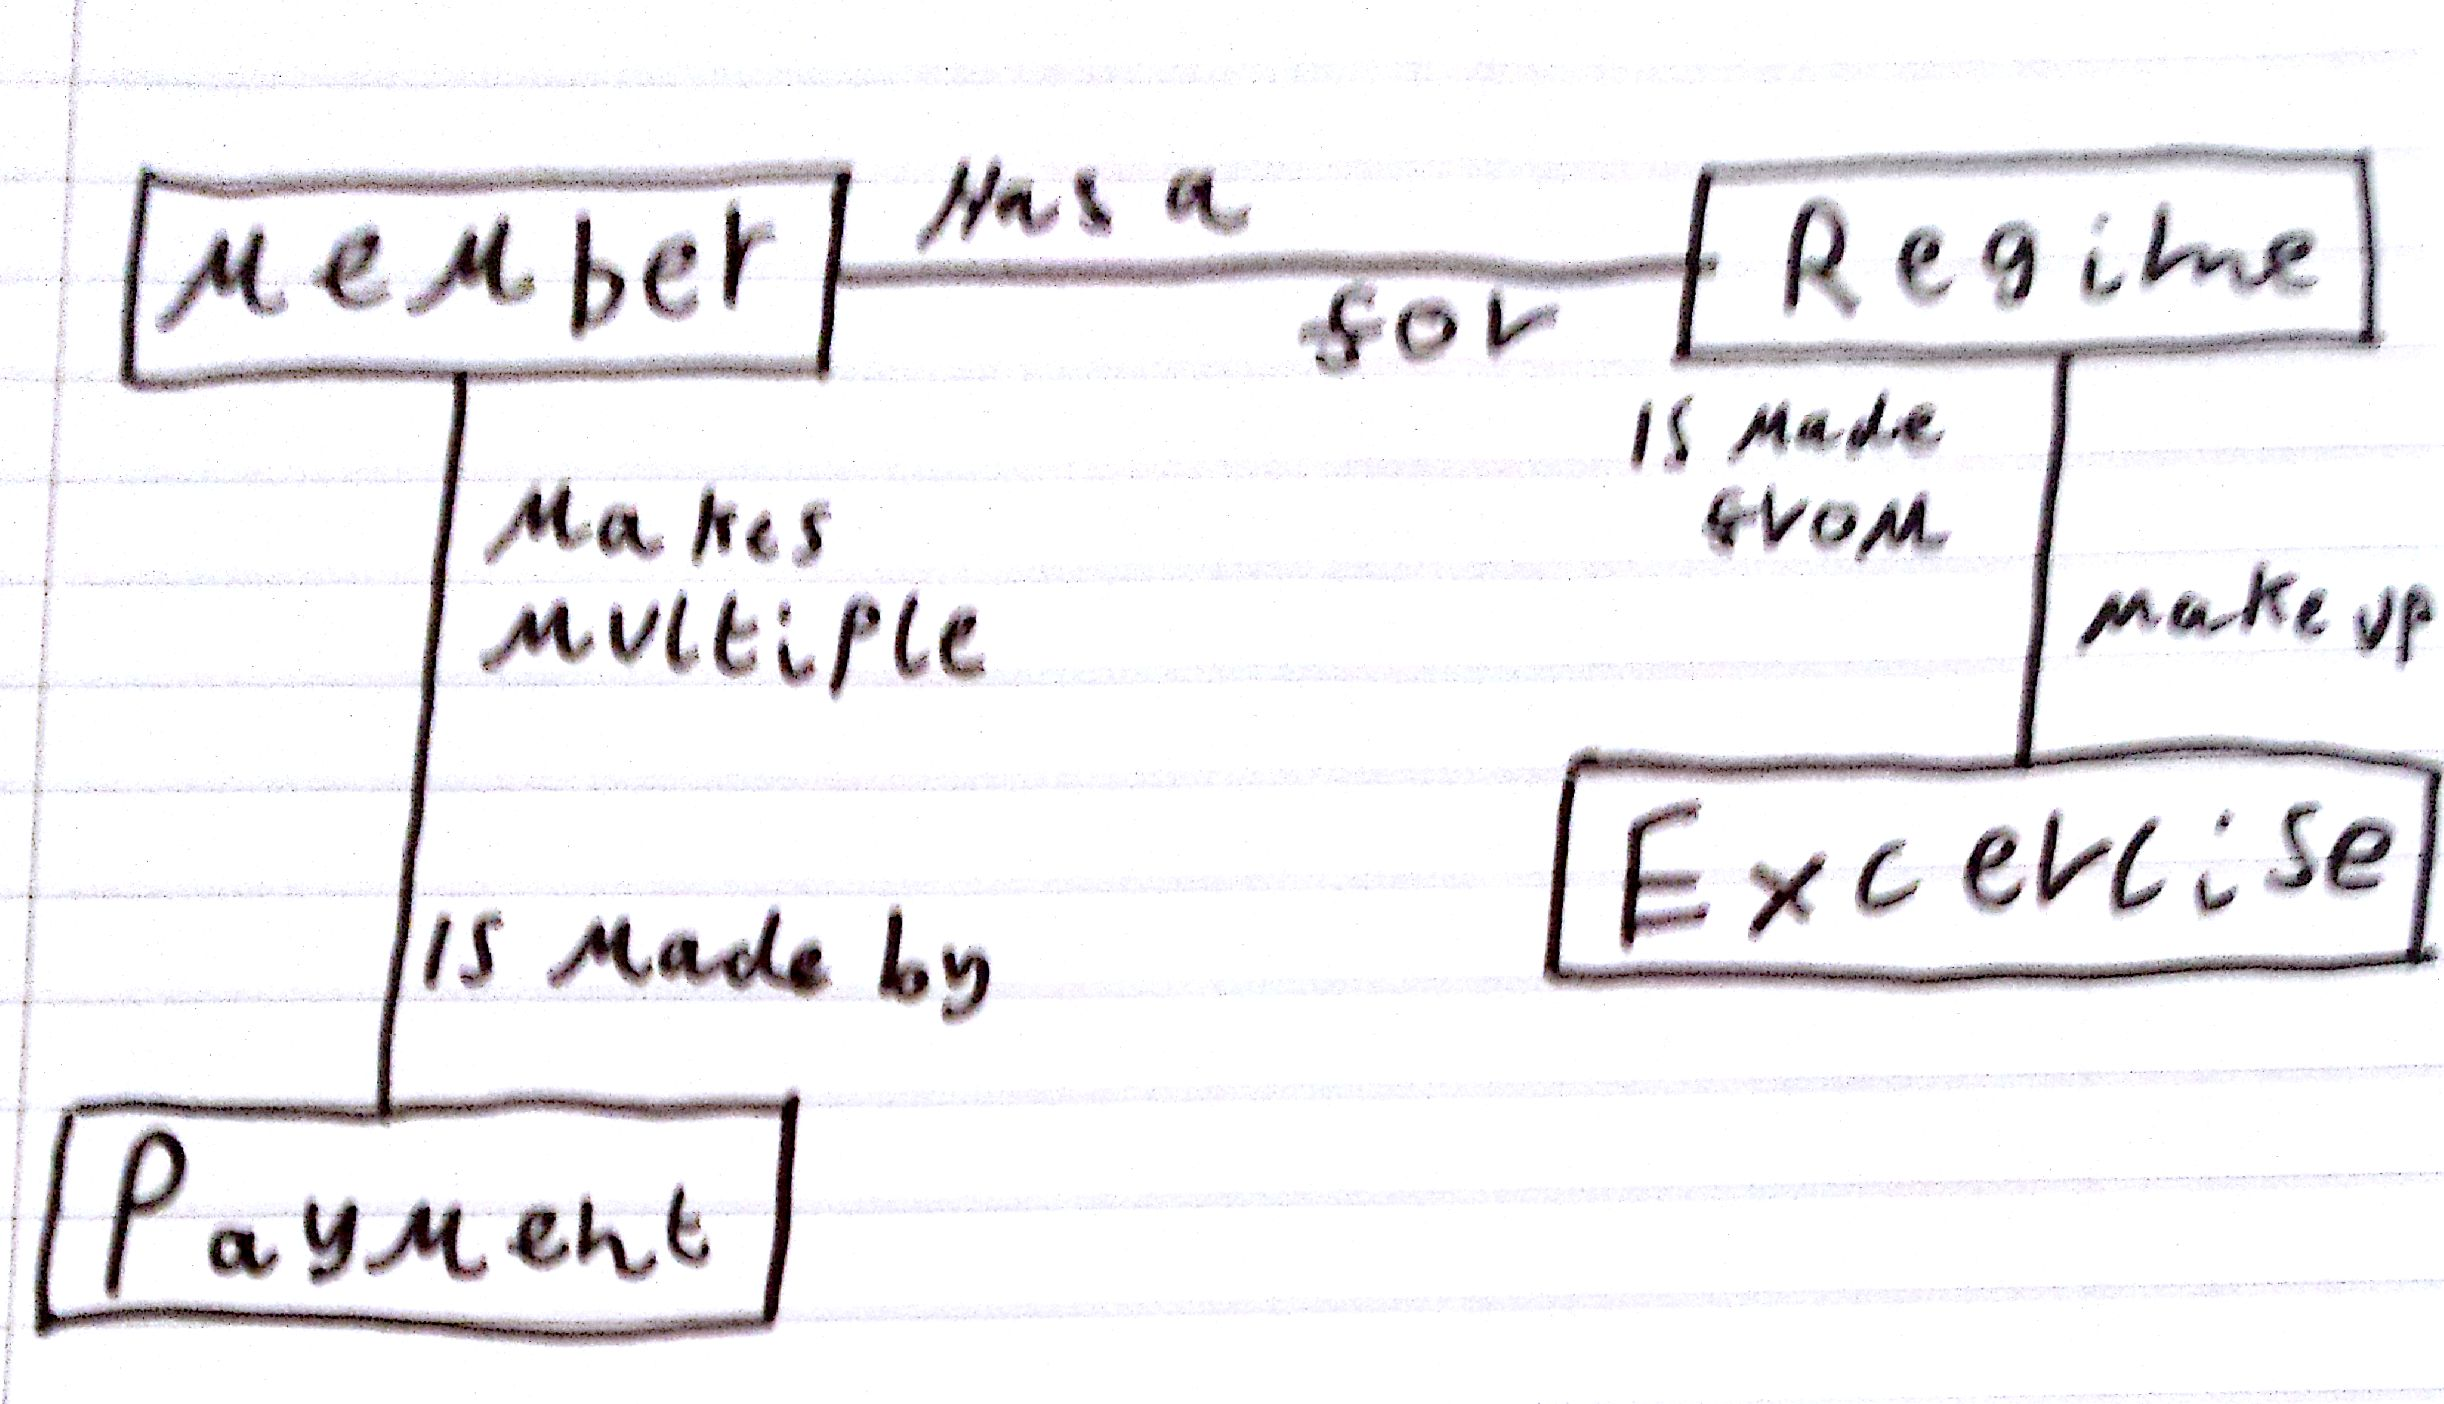
\includegraphics[width=\textwidth]{RelationshipDiagram.jpg}
    \caption{Relationship Diagram} \label{fig: Relationship Diagram}
\end{figure}

\subsection{Class definitions}

\begin{figure}[H]
    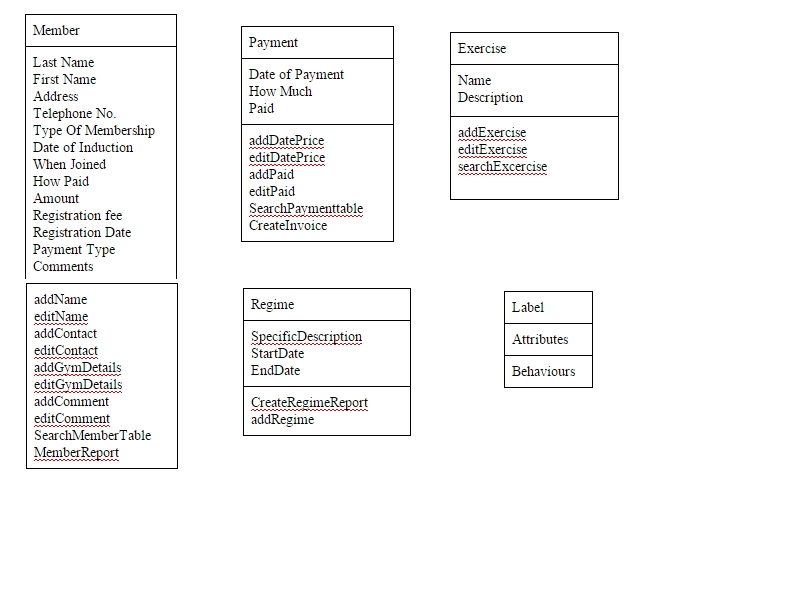
\includegraphics[width=\textwidth]{ClassDefinitions.JPG}
    \caption{Definitions} \label{fig: Definitions}
\end{figure}

\section{Other Abstractions and Graphs}

\begin{figure}[H]
    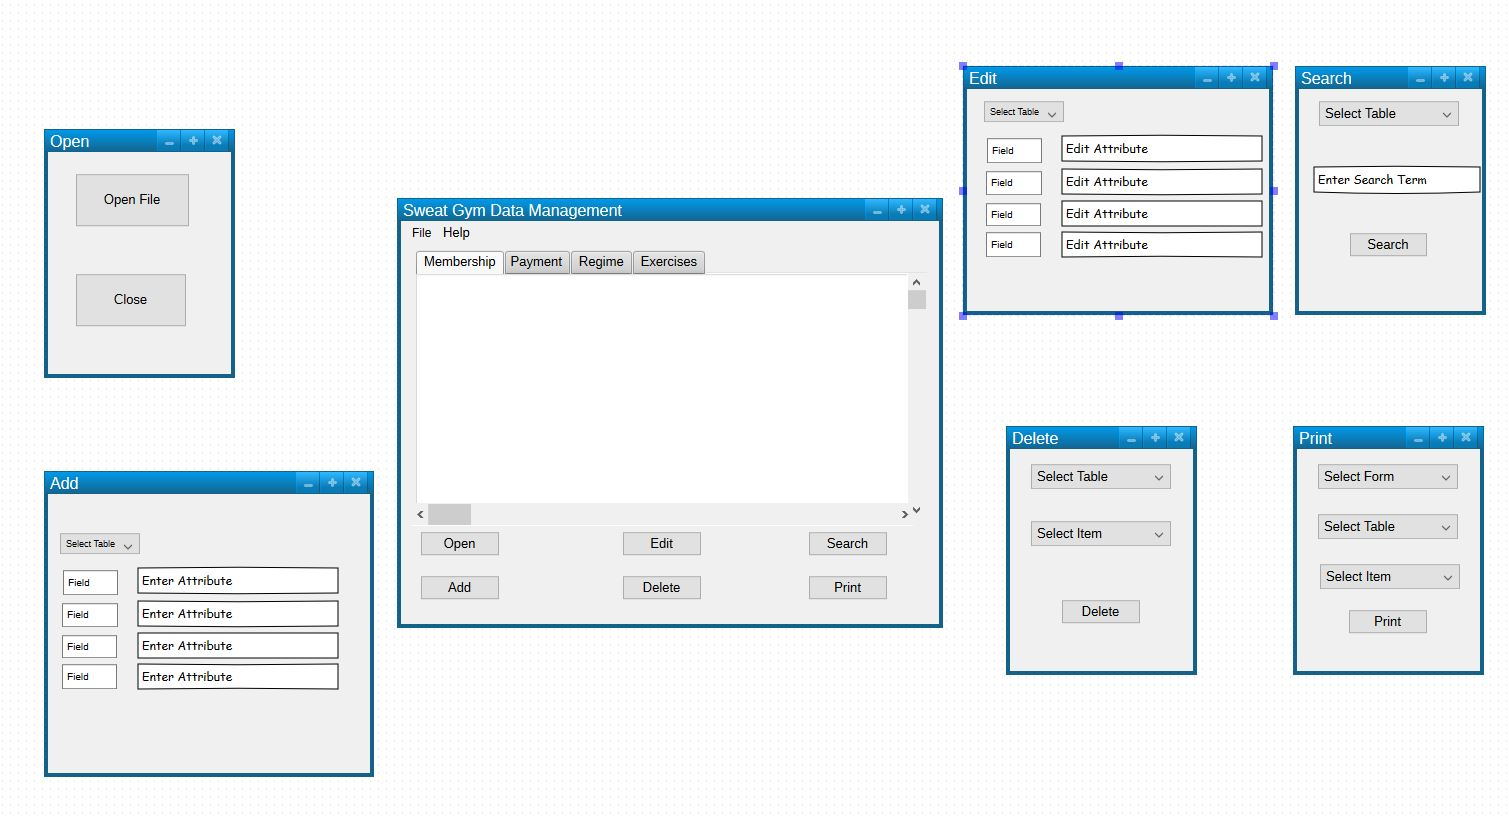
\includegraphics[width=\textwidth]{GUI_DESIGNS.JPG}
    \caption{This is the early preliminary designs for the GUI for the proposed system. It shows a main window (with a white box representing where the database will be presented) containing 6 push buttons that open into the 6 respective dialog boxes.} \label{fig: Preliminary Gui Mockup Presented to Client}
\end{figure}



\section{Constraints}

\subsection{Hardware}

The owner currently uses a Notebook laptop powered by an intel 1st generation i5 processor and 4GB of RAM. He already uses this laptop to run his current system which uses more resources and power than this system will hopefully require, but if not he still has more than enough horse power to run the new system. His use of a laptop is convienient as it means his system is portable so he doesn't need to do any data entry (if required) confined to his office and away from his client if he doesn't want too and it also means he has a battery so in the case of a power outtage he wont lose any data. Though it is worth noting that he may soon be upgrading to a more powerful desktop soon so while this lowers portability, he has more power for the proposed system and he can easily have a battery backup in the form of a UPS(Uninterptable Power Supply).

All members will be running this program off the same workstation so the databases don't need to be primarily stored online and stored locally as the files don't need to be portable. This also adds a level of security.

The only hardware constraint this laptop proposes is the size and resolution of the screen. As it is only 1440p x 900p and 15 inches diagonally this doesn't give him much room to observe over 1300 clients without excessive amounts of scrolling. Fortunately this could be easily solved by either upgrading to a desktop or simply using an external monitor of a higher resolution.

\subsection{Software}

My client has no preference on what software can or cannot be used as long as its easily accessable to him as he isn't the most computer literate person. Its worth noting that although he has no particular requirements for software he isn't willing to learn a new operating system so it will have to run on windows 7. This is not a problem since the proposed system will be developed on a windows os and should be fully compatable. The client wants the system to be secure so the databases are going to be programmed in SQL and the system itself is going to have two levels of password protection including password protecting the SQL database.

\subsection{Time}

My client has given me no personal deadline for this project so the only one I have is the one set by AQA which at the time of writing is April 2015. Although my client doesn't need the new system immediately he is willing to use it as soon as possible and willing to test it before its finished providing its in a fully functioning state.

\subsection{User Knowledge}

Although the owner and staff members aren't specifically trained in I.T they are all completely able to use a computer when given the necessary instruction and support. Most of the staff only use computers for email and web browsing, and occasioinally writing things with a word processing package, as well as the current system which is computer based.

\subsection{Access restrictions}

Access to the proposed system should only be available to members of sweat gymnasium staff and thus the system may need a password although my client insists that only authorised people will have access to the computer, which is password protected itself so the password may be set to optional incase he wants to deactiate it. Due to the system containing private and confidential data on individuals it will have to comply with the Data Protection Act and appropriate action will be taken to do so though the care of the programs security is mostly in the hands of the staff and owner. Although the password for the program may be made optional I insisted that the database be password protected so that people without clearance can't open the database in another browser for malicious or freudulant purposes. If a password is used for the program which it likely will be then a secondary password will be used for the delete option so that no novice users can accidentally delete an item as only higher users who are authorised (like the manager) will have access to that password.

\section{Limitations}

\subsection{Areas which will not be included in computerisation}

For the less technically inclined who don't have email or don't feel that digital forms are of convienience there will be physical forms for them to fill out that would then require their data to be entered into the proposed system manually by the owner or a member of staff. The forms that need to be filled out to determine an exercise regime/programme will also stay physical as they have some very specific questions that can't easily be answered with enough detail in a digital form since the applying member may need assistance from a member of staff and consultation from a trainer. 

\subsection{Areas considered for future computerisation}

Although the invoices and printout records of each member could be stored digitally this would be a bad idea for a number of reasons. First of all the printouts could need updating at anytime and if they need a new physical record the gym will need an up to date one instead of an older one they saved from a couple of months before. Another reason for this is that Iv'e been told by the owner that he would prefer to keep hard copies of invoices over digital so that he not only has a physical record of the invoice for accountancy reasons and so he can send one to any of his clients, even the ones with little computer knowledge. The forms also change repeatedly so if they were saved an older version could be printed out instead by accident. This will be considered for future computerisation as it may come in handy if the owner decides he may want digital copies of forms kept if he believes hes going to need to repeatedly print off an unchanged form in the future, or needs a digital record of a table in a previous state. So a fucntion to save a form to a text file or binary file that can be reread by the program to be printed off in the future may be added.  

\section{Solutions}

\subsection{Alternative solutions}

Improving Spreadsheets
\begin{itemize}
    \item Advantages
    \begin{itemize}
        \item More familiar structure to the current system
        \item Easier to edit to adapt to new features
        \item Easy to make back ups
        \item Microsoft support available if anything goes wrong with the software
        \item Gets rid of all the data duplication in the current spreadsheets
    \end{itemize}
    \item Disadvantages
    \begin{itemize}
        \item Still prone to the same security issues as the old system
        \item All data still has to be entered manually
        \item No easy and specific way to sort through data
        \item No easy to create invoices or printable records
    \end{itemize}
\end{itemize}

Online HTML Based Application

\begin{itemize}
    \item Advantages
    \begin{itemize}
        \item Easy to access using any computer running any operating system and even mobile devices
        \item Low system requirements as it runs in browser based on HTML
        \item Cloud based so backups can be kept securely on error checking hardware/servers
        \item SQL has great web integraion for databases
        \item Wouldn't require that anything would need to be installed
    \end{itemize}
    \item Disadvantages
    \begin{itemize}
        \item I don't know HTML/CSS and javascript that well and would have to spend large amounts of development time learning the language
        \item Online applications have massive sequrity risks and ths could open the sytem up to attacks like SQL injection
        \item If the gyms internet connection becomes innadequate for any reason then he system couldn't be accessed
        \item Web hosting can be very expensive 
    \end{itemize}
\end{itemize}

Paper Based Manual System

\begin{itemize}
	\item Advantages
	\begin{itemize}
		\item Easy for everyone to understand as it requires no technology
		\item Can be used immediately as there will be basically no development time
	\end{itemize}
	\item Disadvantages
	\begin{itemize}
		\item Requires a large amount of space to store so many physical documents
		\item No easy way of making backups except for maybe carbon copies
		\item Can easily be damaged and destroyed/lost
		\item Has no easy search method and could easily become un-organised
		\item No way to edit documents
	\end{itemize}
\end{itemize}

Command Line Application Programmed in Python implementing a database saved to text or binary files

\begin{itemize}
	\item Advantages
	\begin{itemize}
		\item Relatively easy to program with a short development time
		\item Easy to use if users are taught appropriately
		\item Can be programmed to do anything required and easily modified in the future
		\item Saving the databases to one of these formats is relatively easy to programm and manage.
	\end{itemize}
	\item Disadvantages
	\begin{itemize}
		\item Commandline can be difficult for some people to understand 
		\item Executing the program may be difficult for some users
		\item Using text files and binary files is very insecure as they can be easily edited, manipulated and read by anyone with moderate I.T knowledge.
		\item Using these formats means that all sorting methods and search methods have to be programmed be me instead of using a function from a library like sqlite3 resulting in a considerable use of time and resources that isn't necessary.
	\end{itemize}
\end{itemize}

Command Line Application Programmed in Python implementing a database programmed and managed in SQL

\begin{itemize}
	\item Advantages
	\begin{itemize}
		\item Relatively easy to program with a short development time
		\item Easy to use if users are taught appropriately
		\item Can be programmed to do anything required and easily modified in the future
		\item Uses relational databases that will be easily understandable as it will be designed to my clients specifications when compared to the previous excel spreadsheets as well as being more secure than a text or binary file as well as being easier to manipulate with the sqlite3 library.
		\item With the database being saved as a database file, if the program encounters some form of unkown bug down the line the database can still be opened using another SQL browser program
	\end{itemize}
	\item Disadvantages
	\begin{itemize}
		\item Commandline can be difficult for some people to understand 
		\item Executing the program may be difficult for some
		\item SQL is slightly more difficult to programm compared to just using text files or binary files
	    \item SQL still isn't totally secure as using digital input forms means that it may be susceptable to SQL injection and other security faults.
	\end{itemize}
\end{itemize}

GUI Based Application Programmed in Python using the PyQt Library implementing a database programmed and managed in SQL.

\begin{itemize}
	\item Advantages
	\begin{itemize}
		\item Easy to program as I have experience with both python and PyQt so the development time will be quite short
		\item Can be programmed to do anything the client requests
		\item Easy to use as entirely GUI based so users only need basic computer knowledge
		\item That program can be made into an executable using cx freeze so its easy to open and doesnt require the install of any additional programs
		\item Can be programmed to do anything required and easily modified in the future
		\item Uses relational databases that will be easily understandable as it will be designed to my clients specifications when compared to the previous excel spreadsheets as well as being more secure than a text or binary file as well as being easier to manipulate with the sqlite3 library.
		\item With the database being saved as a database file, if the program encounters some form of unkown bug down the line the database can still be opened using another SQL browser program
	\end{itemize}
	\item Disadvantages
	\begin{itemize}
	    \item Not as easy an adjustment as updating the current spreadsheets would be
	    \item Not as easy to create as a command line based program
	    \item SQL is slightly more difficult to programm compared to just using text files or binary files
	    \item SQL still isn't totally secure as using digital input forms means that it may be susceptable to SQL injection and other security faults.
	\end{itemize}
\end{itemise}
		

\subsection{Justification of chosen solution}

My Chosen solution is too use an application with a GUI programmed in python with the library PyQt implementing a database programmed and managed in SQL. This is because of a number of reasons:

\begin{itemize}
    \item I am familiar with python and PyQt and know how to use them as well as knowing how to use and disect their documentation if I ever get lost
    \item Python is easy to install and I can easily use it to debug the program on the gyms workstation if needed incase of emergency though the program will be distributed to my client as a executable
    \item If its more accessable to the client I can even make an executable of the program using a program like cx freeze
    \item Programming in python gives me the opportunity to present and demonstrate my knowledge of complex programming features like Object Oriented Programming and recursive programming
    \item Python gives me he flexibility to program the system to my clients exact specification as its a fully featured programming language
    \item The use of relational databases can be implemented using python and the SQLite3 library meaning it will be easy to store and manipulate the data required using SQL as oppossed to just a text file or a binary file or an Excel spreadsheet
    \item The use of SQL databases is that it is much more secure than simply saving the data to a text file, or pickling the data to create a binary file, and even more secure than a password protected or encrypted Excel spreadsheet. It also means that in the event that the program encounters an issue that the database can be opened in another SQL Browser, even if the interface wont be as suited to the clients needs as the one I will have programmed in the chosen solution.
    \item This also means that the database can be presented in any format/design that is desired as long as its possible to program
\end{itemize}